\documentclass[12pt,a4paper]{report}

%------------------------------------------------
% Packages
%------------------------------------------------

\usepackage{iftex}
\ifPDFTeX
\usepackage{times}
\else
% XeTeX / Tectonic: Times-compatible OpenType font
\usepackage{fontspec}
\setmainfont{texgyretermes}[Extension=.otf, UprightFont=*-regular, BoldFont=*-bold, ItalicFont=*-italic, BoldItalicFont=*-bolditalic]
\fi
\usepackage{setspace}
\usepackage{geometry}
\usepackage{graphicx}
\usepackage{titlesec}
\usepackage{fancyhdr}
\usepackage{cite}
\usepackage{url}
\usepackage{subcaption}
\usepackage{xcolor}
\usepackage{pdfpages}
\usepackage{array}
\usepackage{tabularx}
\usepackage{longtable}
\usepackage{float}
\usepackage{enumitem}
\usepackage{amsmath}
\usepackage{listings}

%------------------------------------------------
% Margins
%------------------------------------------------

\geometry{
top=1in,
bottom=1.25in,
left=1.5in,
right=0.8in
}

\onehalfspacing

%------------------------------------------------
% Chapter formatting
%------------------------------------------------

\titleformat{\chapter}
{\bfseries\centering\fontsize{16}{18}\selectfont}
{\thechapter.}{1em}{\MakeUppercase}

\titleformat{\section}
{\bfseries\fontsize{14}{16}\selectfont}
{\thesection}{1em}{}

\titleformat{\subsection}
{\bfseries\fontsize{12}{14}\selectfont}
{\thesubsection}{1em}{}

%------------------------------------------------
% Page Style
%------------------------------------------------
\setlength{\headheight}{40pt}
\pagestyle{fancy}
\renewcommand{\headrulewidth}{0pt}
\fancyhf{}
\fancyfoot[C]{\thepage}
\fancypagestyle{frontpages}{
\fancyhf{}
\fancyhead[C]{
\includegraphics[width=\textwidth]{sitheader.png}}
\fancyfoot[C]{\thepage}
\renewcommand{\headrulewidth}{0pt}
}

\definecolor{sitred}{RGB}{175,037,028}

%------------------------------------------------
% Table and code helpers
%------------------------------------------------
\newcolumntype{L}{>{\raggedright\arraybackslash}X}
\newcolumntype{P}[1]{>{\raggedright\arraybackslash}p{#1}}
\renewcommand{\arraystretch}{1.25}
\setlist{itemsep=2pt,topsep=4pt}

\lstset{basicstyle=\ttfamily\footnotesize, breaklines=true, frame=single, columns=fullflexible,
        keywordstyle=\bfseries, showstringspaces=false}

% Placeholder page for documents that must be inserted later
\newcommand{\placeholderpage}[2]{%
\begin{center}
\vspace*{3cm}
\fbox{\parbox{0.85\textwidth}{\centering\vspace{1cm}
{\large\textbf{#1}}\\[0.6cm]
#2\vspace{1cm}}}
\end{center}}

% Primitive \input, so generated table rows do not leave an empty row at the end of a tabular
\makeatletter\newcommand{\tabinput}[1]{\@@input #1 }\makeatother

% Numbers from the latest training run (written by scripts/report_assets.py)
\newcommand{\BestModel}{Logistic Regression}
\newcommand{\BestCVAUC}{0.839}
\newcommand{\BestOOFAUC}{0.843}
\newcommand{\BestTestAUC}{0.813}
\newcommand{\BestAcc}{84.6}
\newcommand{\BestPrec}{52.6}
\newcommand{\BestRecall}{55.6}
\newcommand{\BestFone}{54.0}
\newcommand{\BestThr}{0.68}
\newcommand{\BestRecallHalf}{75}
\newcommand{\BestPrecHalf}{42}
\newcommand{\CmTN}{167}
\newcommand{\CmFP}{18}
\newcommand{\CmFN}{16}
\newcommand{\CmTP}{20}
\newcommand{\TestLeavers}{36}
\newcommand{\TestRows}{221}
\newcommand{\DevRows}{1249}
\newcommand{\DevLeavers}{201}
\newcommand{\TestRowsSplit}{221}
\newcommand{\AttrRate}{16.1}
\newcommand{\Leavers}{237}
\newcommand{\OTYes}{30.5}
\newcommand{\OTNo}{10.4}
\newcommand{\SingleRate}{25.5}
\newcommand{\MarriedRate}{12.5}
\newcommand{\TopRole}{Sales Representative}
\newcommand{\TopRoleRate}{39.8}
\newcommand{\LowRole}{Research Director}
\newcommand{\LowRoleRate}{2.5}
\newcommand{\TopFeature}{YearsSinceLastPromotion}


\newcommand{\projtitle}{Employee Attrition Prediction using HR Analytics}
\newcommand{\repourl}{https://github.com/varunmundhada/employee-attrition-prediction}

%------------------------------------------------
\begin{document}

%================================================
% COVER PAGE
%================================================

\begin{titlepage}

\begin{center}

\vspace{0.5cm}

\fontsize{24}{20}\textcolor{sitred}{\textbf{Symbiosis Institute of Technology, Nagpur}}\\

\vspace{0.7cm}

{\fontsize{18}{20}\selectfont \textbf{PROJECT REPORT}}

\vspace{0.4cm}

{\fontsize{15}{18}\selectfont \textit{\projtitle}}

\vspace{0.3cm}

{\fontsize{13}{16}\selectfont Industry Domain: \textbf{HR Analytics}}

\vspace{0.5cm}

Submitted in partial fulfillment of requirement for the award of degree of

\vspace{0.5cm}

{\fontsize{16}{18}\selectfont \textbf{Bachelor of Technology}}

in

{\fontsize{16}{18}\selectfont \textbf{Computer Science and Engineering}}

\vspace{0.5cm}

by

\vspace{0.5cm}

{\fontsize{14}{16}\selectfont \textbf{Varun Mundhada}}

PRN: 23070521184

\vspace{0.8cm}

{\fontsize{13}{16}\selectfont Course: \textbf{Big Data Analytics} (Course Code: 0705210731)\par}

{\fontsize{12}{15}\selectfont Academic Year: 2026-27 \quad | \quad Batch: 2023-27\par}

\vspace{0.6cm}

Under the guidance of\\
\vspace{0.4cm}
{\fontsize{16}{18}\selectfont \textbf{Dr. Dharamveer Chaudhary}}\\
Institute Guide, Department of Computer Science and Engineering

\vspace{0.6cm}

{\fontsize{16}{18}\selectfont \textbf{October 2026}}

\vspace{0.5cm}

\includegraphics[width=1.5cm]{siulogo.png}

\vspace{0.5cm}
\fontsize{19}{22}\selectfont\textcolor{sitred}{\textbf{Symbiosis International (Deemed University), Pune}}\\

\end{center}

\end{titlepage}

%================================================
% DECLARATION
%================================================
\pagenumbering{roman}
\chapter*{Declaration}
\thispagestyle{frontpages}

I, hereby declare that the project report titled \textbf{``\projtitle''} submitted herein has been carried out by me at the \textbf{Department of Computer Science and Engineering, Symbiosis Institute of Technology, Nagpur} towards partial fulfillment of requirement for the award of Degree of Bachelor of Technology in Computer Science and Engineering. The work is original and has not been submitted earlier as a whole or in part for the award of any degree / diploma at this or any other Institution / University.

\vspace{0.2cm}
I hereby assign all copyright rights in this work, including any revised or expanded derivative works, to Symbiosis Institute of Technology, Nagpur. Any content sourced from references, manuals, datasets or other external materials is duly acknowledged and disclaimed.

\vspace{2cm}

Name of Student: \textbf{Varun Mundhada}

PRN: \textbf{23070521184}

Signature:
\vspace{2cm}

Place: Nagpur

Date: \today

%================================================
% CERTIFICATE
%================================================

\chapter*{Certificate}
\thispagestyle{frontpages}

This is to certify that the project report titled \textbf{``\projtitle''} (Industry Domain: HR Analytics) has been carried out under my supervision by \textbf{Varun Mundhada} (PRN: 23070521184) in partial fulfillment of the requirements for the Bachelor of Technology in Computer Science and Engineering. The work submitted is comprehensive, complete and fit for evaluation.
\vspace{2.5cm}

\textbf{Dr. Dharamveer Chaudhary} \hfill \textbf{Dr. Sagarkumar S. Badhiye}

Institute Guide \hfill Head of Department

\vspace{2.5cm}

\begin{center}
\textbf{Dr. Nitin Rakesh}\\
Professor and Director
\end{center}

%================================================
% ACKNOWLEDGEMENT
%================================================

\chapter*{Acknowledgement}
\thispagestyle{frontpages}

I express my sincere gratitude to my institute guide, \textbf{Dr. Dharamveer Chaudhary}, for the guidance, feedback and encouragement throughout this project, carried out for the course Big Data Analytics (0705210731). The suggestions on the problem definition and on how to evaluate the models shaped the final work.

I extend my heartfelt appreciation to our Director, \textbf{Dr. Nitin Rakesh}, for his continuous support in providing students with the resources and environment for project work. I would also like to express my deepest gratitude to \textbf{Dr. Sagarkumar S. Badhiye}, Head of the Department, Computer Science and Engineering, for his constant support and guidance throughout my academic journey.

I thank the faculty members of the Department of Computer Science and Engineering, whose courses in data structures, database systems, machine learning and big data analytics gave me the foundation for this project. I also acknowledge IBM for publishing the HR Analytics Employee Attrition dataset, and the Apache Spark and Streamlit open-source communities whose tools made this project possible.

I used AI writing tools to help structure and draft parts of this report. The design, code, experiments and results described in it are my own.

Lastly, I would like to acknowledge my family and friends for their unwavering support and encouragement.

\vspace{1cm}
\hfill \textbf{Varun Mundhada}

%================================================
% ABSTRACT
%================================================

\chapter*{Abstract}
\thispagestyle{frontpages}

Employee attrition, the loss of employees through resignation, is one of the most costly problems an organisation's human resources (HR) function faces. Each departure brings hiring and training costs, lost productivity and lost knowledge, and HR teams usually learn of the risk only when the resignation letter arrives. This project builds a system that predicts which employees are likely to leave, explains why, and gives HR the information early enough to act.

The work uses the IBM HR Analytics Employee Attrition dataset of 1,470 employees and 35 attributes, of whom \Leavers{} (\AttrRate\%) left the organisation. The data is processed with \textbf{Apache Spark}: PySpark DataFrames and Spark SQL are used for cleaning and exploratory analysis, and a \textbf{Spark MLlib} pipeline performs feature engineering, categorical encoding, scaling and classification. Four classifiers, Logistic Regression, Decision Tree, Random Forest and Gradient-Boosted Trees, are tuned with 5-fold cross-validation on a stratified training set, with class weights to handle the imbalance between leavers and stayers. The decision threshold is chosen from out-of-fold predictions, the model with the best cross-validated AUC is selected, and the result is evaluated once on an untouched, stratified test set.

The best model, \textbf{\BestModel}, reached a test ROC-AUC of \textbf{\BestTestAUC}, with a recall of \BestRecall\% and an F1-score of \BestFone\% for employees who left. The analysis confirms overtime, low income and job level, short tenure, low stock-option level, single marital status and low satisfaction as the strongest signals of attrition. Employees working overtime leave at \OTYes\% against \OTNo\% for those who do not. A scalability test on synthetically enlarged data up to about 735,000 records shows that the same Spark pipeline runs unchanged at a much larger scale.

The trained model is deployed in a \textbf{Streamlit} web application with an HR dashboard, single-employee prediction with a what-if explanation of the risk drivers and suggested HR actions, batch scoring of CSV files, and a model-performance page. The complete source code is published on GitHub.

\vspace{0.5cm}
\noindent\textbf{Keywords:} Employee attrition, HR analytics, Apache Spark, Spark MLlib, machine learning, gradient-boosted trees, class imbalance, Streamlit.

%================================================
% CONTENTS
%================================================

\clearpage
\tableofcontents
\clearpage
\listoffigures
\clearpage
\listoftables

\chapter*{List of Abbreviations}
\addcontentsline{toc}{chapter}{List of Abbreviations}

\begin{table}[H]
\centering
\begin{tabularx}{0.85\textwidth}{|P{3cm}|L|}
\hline
\textbf{Abbreviation} & \textbf{Full form} \\ \hline
AUC & Area Under the (ROC) Curve \\ \hline
CSV & Comma-Separated Values \\ \hline
CV & Cross-Validation \\ \hline
DT & Decision Tree \\ \hline
EDA & Exploratory Data Analysis \\ \hline
FN / FP & False Negative / False Positive \\ \hline
GBT & Gradient-Boosted Trees \\ \hline
HR & Human Resources \\ \hline
LR & Logistic Regression \\ \hline
MLlib & Apache Spark's Machine Learning Library \\ \hline
PR & Precision--Recall \\ \hline
RDD & Resilient Distributed Dataset \\ \hline
RF & Random Forest \\ \hline
ROC & Receiver Operating Characteristic \\ \hline
SQL & Structured Query Language \\ \hline
TN / TP & True Negative / True Positive \\ \hline
\end{tabularx}
\end{table}

\clearpage
\pagenumbering{arabic}

%================================================
% CHAPTER 1: INTRODUCTION
%================================================

\chapter{Introduction}

\section{Background}

People are the largest cost and the most important asset of most organisations. When an employee leaves, the organisation pays to advertise the role, interview candidates, onboard and train the replacement, and absorb months of reduced productivity while the new person learns the job. Studies of turnover put the full cost of replacing an employee at a large fraction of that employee's annual salary, and higher still for skilled and senior roles \cite{allen2010retaining}. Departures also carry costs that are harder to measure: knowledge leaves with the employee, workloads rise for the colleagues who stay, and repeated exits lower team morale.

\textbf{HR analytics}, also called people analytics, applies data analysis to workforce decisions. Organisations already hold the data needed to understand attrition: demographic details, job role and level, compensation, overtime, travel, tenure, promotion history, performance ratings and satisfaction surveys. Analysed together, these records show patterns that are not visible when each employee is considered on their own. Machine learning takes the next step: it learns those patterns from past leavers and stayers and uses them to estimate the risk for each current employee.

\section{Motivation}

Most organisations react to attrition rather than prevent it. HR usually learns that someone is unhappy only when they resign, and by then the decision is made. A model that ranks employees by their risk of leaving lets HR focus retention effort, such as stay interviews, compensation reviews, workload changes or career discussions, on the people most likely to leave, while there is still time to act.

Two further points shaped this project. First, a risk score alone does not tell HR what to do. The system must explain \emph{why} an employee is at risk, so that the action matches the cause. Second, HR data grows with the organisation and is often combined with attendance, survey and system-log data. The processing should therefore be built on a platform that scales, which is why this project uses \textbf{Apache Spark} rather than a single-machine library.

\section{Problem Statement}

\textit{Given the HR records of an organisation's employees, predict for each employee whether they are likely to leave the organisation, identify the factors that drive that risk, and present the predictions and insights to HR users through an easy-to-use application, using a scalable big-data processing pipeline.}

The problem is a supervised binary classification task with an imbalanced target: only about one employee in six leaves, so a model that simply predicts ``stays'' for everyone would be 84\% accurate and completely useless. The evaluation must therefore focus on how well the model finds the leavers (recall), how many of its warnings are correct (precision), and how well it ranks employees by risk (ROC-AUC).

\section{Objectives}

\begin{enumerate}
\item To analyse the IBM HR Analytics dataset with Apache Spark (PySpark and Spark SQL) and identify the factors associated with employee attrition.
\item To build a reusable Spark MLlib pipeline for cleaning, feature engineering, encoding and scaling of HR records.
\item To train, tune and compare four classification algorithms (Logistic Regression, Decision Tree, Random Forest and Gradient-Boosted Trees), handling the class imbalance between leavers and stayers.
\item To select the best model and decision threshold using only the development data, and report an unbiased evaluation on a held-out test set.
\item To explain individual predictions in terms HR can act on, and map each risk driver to a suggested retention action.
\item To deploy the model in a working web application for single and batch predictions, and to show that the pipeline scales to larger data.
\end{enumerate}

\section{Scope of the Project}

The project covers the full path from raw data to a working application: data analysis, model development, evaluation, explanation, deployment and documentation. It uses a public, anonymised dataset, so no real employee data is involved. The application runs on a single machine with Spark in local mode. The same code runs on a Spark cluster without change, but cluster deployment, integration with a live HR information system and scheduled retraining are outside the scope and are listed as future work.

\section{Organisation of the Report}

Chapter 2 reviews published work on attrition prediction and on Apache Spark. Chapter 3 describes the dataset and the exploratory analysis. Chapter 4 explains the methodology and system design. Chapter 5 describes the implementation and the web application. Chapter 6 presents and discusses the results, and Chapter 7 concludes with future scope. Screenshots and instructions for running the project are in the appendices.

%================================================
% CHAPTER 2: LITERATURE REVIEW
%================================================

\chapter{Literature Review}

\section{Employee Turnover and its Causes}

Research on turnover has long separated its causes into job-related factors (pay, workload, role, promotion, relationship with the manager), personal factors (age, marital status, career stage) and organisational factors (culture, environment, policies). Allen, Bryant and Vardaman \cite{allen2010retaining} review the evidence behind common retention practices. They show that turnover is costly, that it can be predicted from measurable factors, and that the right intervention depends on why a particular group of employees leaves. That last finding is the reason this project explains each prediction instead of only producing a score.

\section{Machine Learning for Attrition Prediction}

Saradhi and Palshikar \cite{saradhi2011employee} framed employee churn as a classification problem, similar to customer churn, and compared naive Bayes, support vector machines, logistic regression, decision trees and random forests. They found that the support vector machine performed best on their data and that churn models are useful only if they are evaluated on the minority class, not on overall accuracy.

Alao and Adeyemo \cite{alao2013analyzing} used decision-tree algorithms (C4.5, C5.0, REPTree and CART) on records from a Nigerian institution and produced readable rules that link salary, length of service and age to attrition. Their work showed the value of interpretable models for HR users.

Punnoose and Ajit \cite{punnoose2016prediction} compared seven classifiers on HR data from a global retailer and found that Extreme Gradient Boosting (XGBoost) gave the best results and was robust to noisy data, an early sign that boosted trees suit this problem.

Zhao et al. \cite{zhao2019employee} ran a large comparison of ten supervised algorithms on small, medium and large HR datasets, including the IBM dataset used in this project. Gradient-boosted tree ensembles were the most reliable across datasets, while simpler linear models stayed competitive on small data.

Fallucchi et al. \cite{fallucchi2020predicting} analysed the same IBM dataset in detail. They studied the relationship of each attribute with attrition and compared Gaussian naive Bayes, logistic regression, k-nearest neighbours, decision tree, random forest and support vector machine classifiers. They found overtime, monthly income, total working years and age among the strongest predictors, and reported that naive Bayes gave the best recall.

Yahia, Hlel and Colomo-Palacios \cite{yahia2021big} looked at attrition prediction from a big-data angle. They argued that people analytics should move ``from big data to deep data'' by combining many HR data sources, and showed that ensemble models with feature selection improve prediction on the IBM data and on larger datasets.

\section{Handling Class Imbalance}

All of the studies above work with data where leavers are a minority. Common remedies are oversampling the minority class, for example with SMOTE \cite{chawla2002smote}, undersampling the majority class, or weighting the classes in the loss function. Class weighting changes no records and works natively with every Spark MLlib classifier used here, so this project weights each leaver by the ratio of stayers to leavers.

\section{Apache Spark and MLlib}

Apache Spark \cite{zaharia2016spark} is a unified engine for large-scale data processing. It keeps data in memory across a cluster and offers one API for SQL, streaming, graph processing and machine learning, which made it the standard successor to Hadoop MapReduce. Spark MLlib \cite{meng2016mllib} is its machine-learning library. It provides distributed implementations of common algorithms and, through its \texttt{Pipeline} API, a way to chain feature transformers and an estimator into one object that can be tuned, saved and reused. Building the attrition model as an MLlib pipeline means the same code can train on the 1,470-record dataset on a laptop or on millions of records on a cluster.

\section{Algorithms Used}

\textbf{Logistic Regression} models the log-odds of leaving as a weighted sum of the features. It is fast, its coefficients are readable, and with elastic-net regularisation it guards against overfitting. \textbf{Decision Trees} split the data on one feature at a time and produce readable rules, but a single tree overfits easily. \textbf{Random Forests} \cite{breiman2001random} average many trees, each grown on a bootstrap sample with a random subset of features, which lowers variance. \textbf{Gradient-Boosted Trees} \cite{friedman2001greedy} build shallow trees one after another, each correcting the errors of the ensemble so far, and are among the strongest methods for tabular data.

\section{Summary and Research Gap}

\begin{table}[H]
\centering
\caption{Summary of the literature reviewed}
\label{tab:lit}
\small
\begin{tabularx}{\textwidth}{|P{3.2cm}|L|L|}
\hline
\textbf{Study} & \textbf{Approach} & \textbf{Key finding} \\ \hline
Saradhi \& Palshikar (2011) & Churn framing; NB, SVM, LR, DT, RF & SVM best; evaluate on the minority class \\ \hline
Alao \& Adeyemo (2013) & C4.5, C5.0, REPTree, CART & Readable rules on salary, service, age \\ \hline
Punnoose \& Ajit (2016) & Seven classifiers incl.\ XGBoost & Boosting best and robust to noise \\ \hline
Zhao et al.\ (2019) & Ten algorithms, three data sizes & Boosted trees most reliable overall \\ \hline
Fallucchi et al.\ (2020) & IBM data; six classifiers & Overtime, income, experience, age key \\ \hline
Yahia et al.\ (2021) & Big data to deep data; ensembles & Ensembles with feature selection improve results \\ \hline
\end{tabularx}
\end{table}

The literature agrees on the main predictors and on the strength of tree ensembles, but most studies stop at a model score computed in a notebook on a single machine. Few of them (i) build the solution on a scalable big-data engine, (ii) separate model and threshold selection from the final test, which is needed for an honest estimate on a dataset this small, (iii) explain each employee's prediction in terms of HR actions, or (iv) deliver a working application HR can use. This project addresses all four.

%================================================
% CHAPTER 3: DATASET AND EXPLORATORY ANALYSIS
%================================================

\chapter{Dataset and Exploratory Data Analysis}

\section{Dataset Description}

The project uses the \textbf{IBM HR Analytics Employee Attrition \& Performance} dataset \cite{ibm_dataset}, created by IBM data scientists to resemble a real organisation's HR records. It has \textbf{1,470 employee records} and \textbf{35 attributes}, and the target column \texttt{Attrition} records whether the employee left (\texttt{Yes}) or stayed (\texttt{No}). There are no missing values. Table~\ref{tab:dict} groups the attributes.

\begin{table}[H]
\centering
\caption{Attributes of the dataset, grouped}
\label{tab:dict}
\small
\begin{tabularx}{\textwidth}{|P{3cm}|L|}
\hline
\textbf{Group} & \textbf{Attributes} \\ \hline
Target & Attrition (Yes / No) \\ \hline
Personal & Age, Gender, MaritalStatus, DistanceFromHome, Education (1--5), EducationField \\ \hline
Job & Department, JobRole, JobLevel (1--5), JobInvolvement (1--4), BusinessTravel, OverTime, PerformanceRating (1--4), TrainingTimesLastYear \\ \hline
Compensation & MonthlyIncome, DailyRate, HourlyRate, MonthlyRate, PercentSalaryHike, StockOptionLevel (0--3) \\ \hline
Satisfaction & EnvironmentSatisfaction, JobSatisfaction, RelationshipSatisfaction (1--4), WorkLifeBalance (1--4) \\ \hline
Tenure & TotalWorkingYears, NumCompaniesWorked, YearsAtCompany, YearsInCurrentRole, YearsSinceLastPromotion, YearsWithCurrManager \\ \hline
Identifiers / constant & EmployeeNumber (ID), EmployeeCount (always 1), Over18 (always Y), StandardHours (always 80) \\ \hline
\end{tabularx}
\end{table}

\section{Data Quality and Cleaning}

The data was loaded into a Spark DataFrame with schema inference. Spark SQL checks found no missing values and no duplicate records. Three columns, \texttt{EmployeeCount}, \texttt{Over18} and \texttt{StandardHours}, hold the same value for every employee and carry no information, so they were removed. \texttt{EmployeeNumber} is kept only as a record identifier for the data split and is not used as a feature. The target was converted to a numeric label (1 = left, 0 = stayed), and all numeric columns were cast to double precision for MLlib. This leaves 23 numeric and 7 categorical input features.

\section{Class Balance}

Of the 1,470 employees, \textbf{\Leavers{} (\AttrRate\%) left} and 1,233 stayed (Figure~\ref{fig:balance}). The imbalance is moderate but important: it is why the project uses class weights, a stratified split, a tuned threshold and AUC / recall / F1 as metrics rather than plain accuracy.

\begin{figure}[H]
\centering
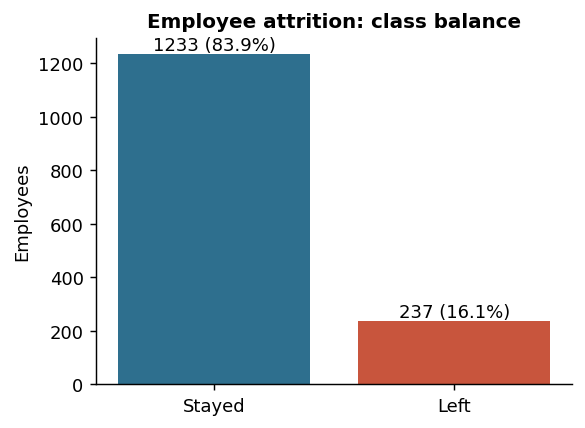
\includegraphics[width=0.55\textwidth]{figures/01_class_balance.png}
\caption{Class balance of the target variable}
\label{fig:balance}
\end{figure}

\section{Exploratory Analysis with Spark SQL}

Each factor was analysed with Spark SQL aggregations of the form \texttt{SELECT factor, COUNT(*), AVG(label) FROM hr GROUP BY factor}. Continuous variables such as age, income and tenure were first grouped into bands with \texttt{CASE WHEN} expressions. In the charts below, bars above the company-wide rate (dashed line) are shown in red.

\textbf{Overtime} is the single strongest categorical signal: employees who work overtime leave at \OTYes\%, almost three times the \OTNo\% rate of those who do not (Figure~\ref{fig:overtime}).

\begin{figure}[H]
\centering
\begin{subfigure}{0.49\textwidth}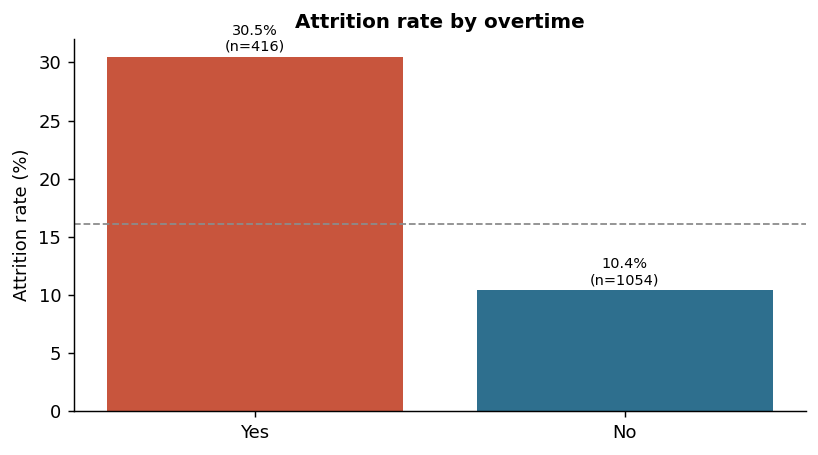
\includegraphics[width=\linewidth]{figures/02_overtime.png}\caption{Overtime}\label{fig:overtime}\end{subfigure}
\begin{subfigure}{0.49\textwidth}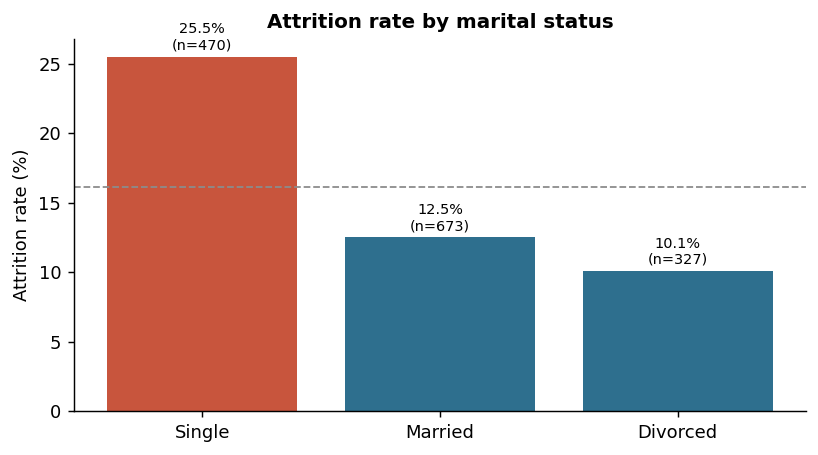
\includegraphics[width=\linewidth]{figures/07_marital.png}\caption{Marital status}\label{fig:marital}\end{subfigure}
\caption{Attrition rate by overtime and marital status}
\end{figure}

\textbf{Job role} matters a great deal (Figure~\ref{fig:role}). \TopRole s leave at \TopRoleRate\%, while \LowRole s leave at only \LowRoleRate\%. Entry-level, lower-paid roles such as laboratory technicians and sales representatives carry the highest risk.

\begin{figure}[H]
\centering
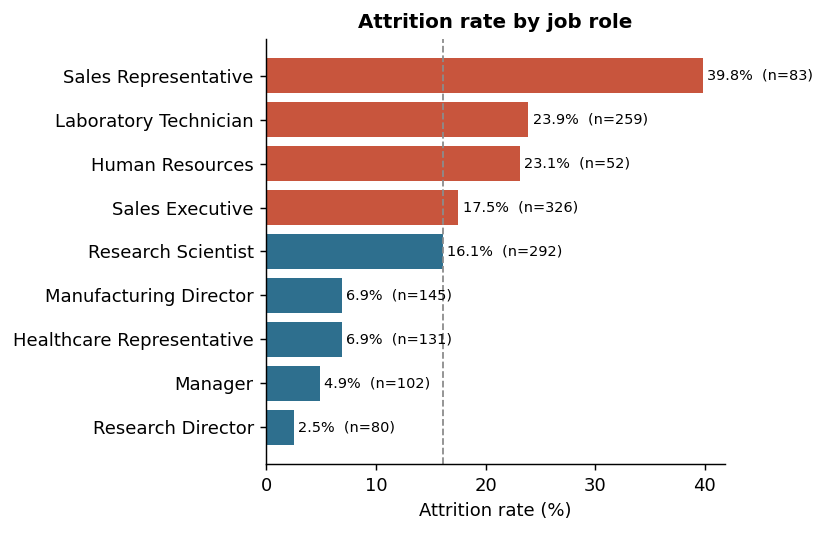
\includegraphics[width=0.75\textwidth]{figures/03_job_role.png}
\caption{Attrition rate by job role}
\label{fig:role}
\end{figure}

\textbf{Income, tenure and age} (Figure~\ref{fig:bands}). Employees earning under 3,000 a month leave at 28.6\%, against 8.9\% for those above 10,000. Attrition is highest in the first two years at the company (34.9\%) and falls steadily with tenure, and employees aged 18--24 leave at 39.2\%. These variables are strongly correlated with each other (Figure~\ref{fig:corr}), and all describe the same group: young, early-career, lower-paid employees.

\begin{figure}[H]
\centering
\begin{subfigure}{0.49\textwidth}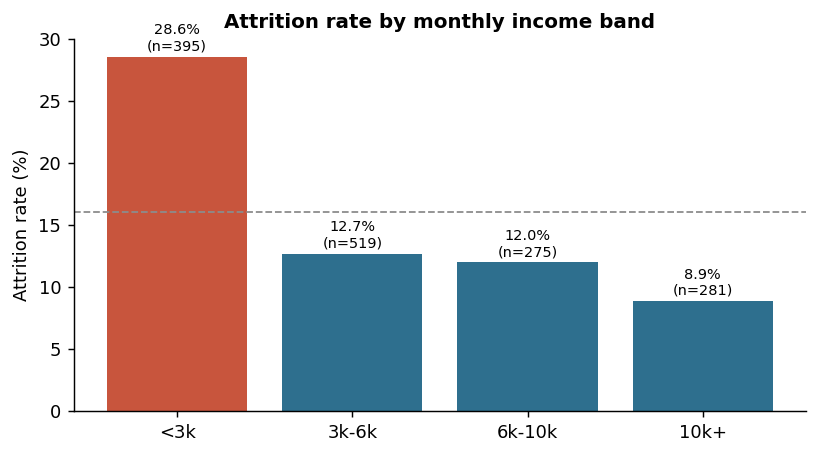
\includegraphics[width=\linewidth]{figures/04_income.png}\caption{Income band}\end{subfigure}
\begin{subfigure}{0.49\textwidth}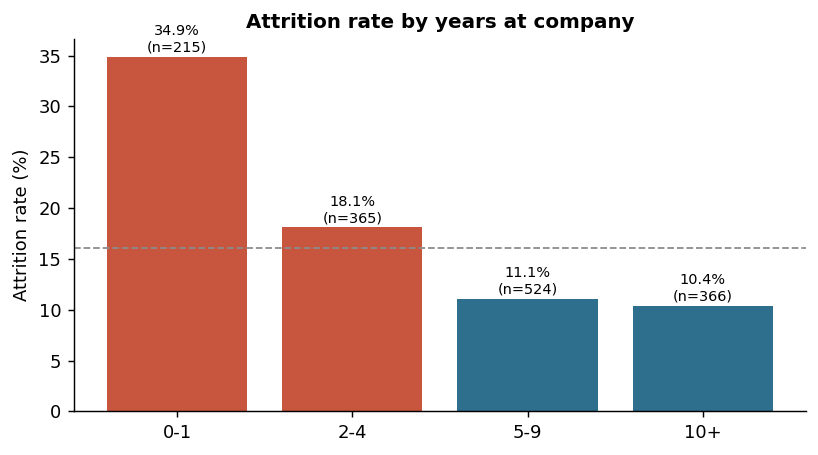
\includegraphics[width=\linewidth]{figures/05_tenure.png}\caption{Years at company}\end{subfigure}
\begin{subfigure}{0.49\textwidth}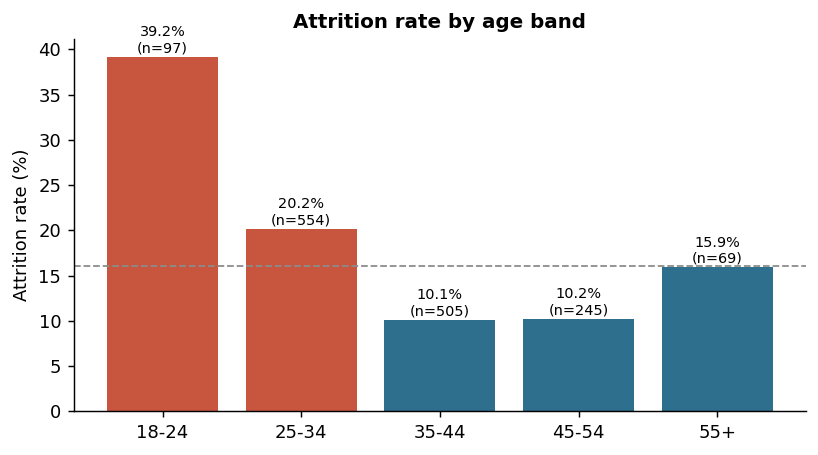
\includegraphics[width=\linewidth]{figures/06_age.png}\caption{Age band}\end{subfigure}
\begin{subfigure}{0.49\textwidth}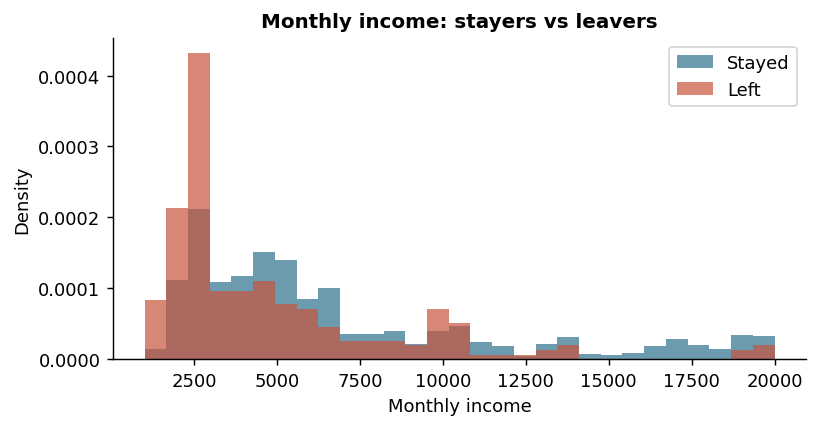
\includegraphics[width=\linewidth]{figures/10_income_distribution.png}\caption{Income distribution}\end{subfigure}
\caption{Attrition by income, tenure and age}
\label{fig:bands}
\end{figure}

\textbf{Marital status, travel and stock options} (Figures~\ref{fig:marital} and~\ref{fig:travelstock}). Single employees leave at \SingleRate\% against \MarriedRate\% for married employees. Frequent travellers leave at 24.9\% against 8.0\% for those who never travel. Employees with no stock options leave at 24.4\%, against 7.6--9.4\% at levels 1 and 2, which suggests long-term incentives help retention.

\begin{figure}[H]
\centering
\begin{subfigure}{0.49\textwidth}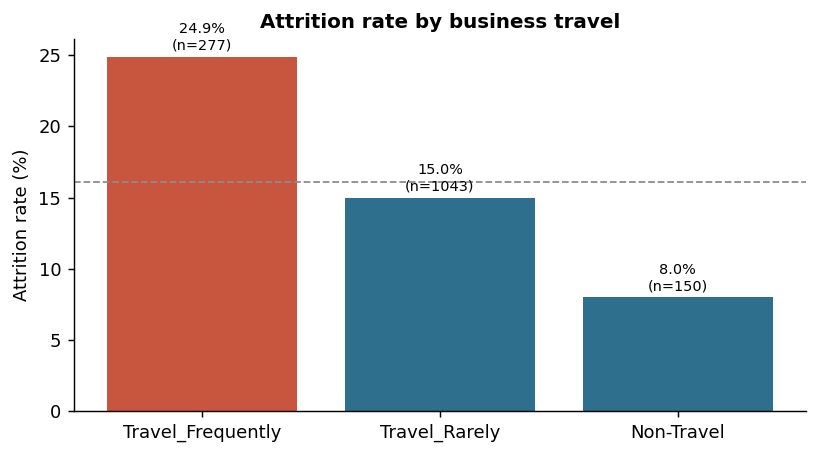
\includegraphics[width=\linewidth]{figures/08_travel.png}\caption{Business travel}\end{subfigure}
\begin{subfigure}{0.49\textwidth}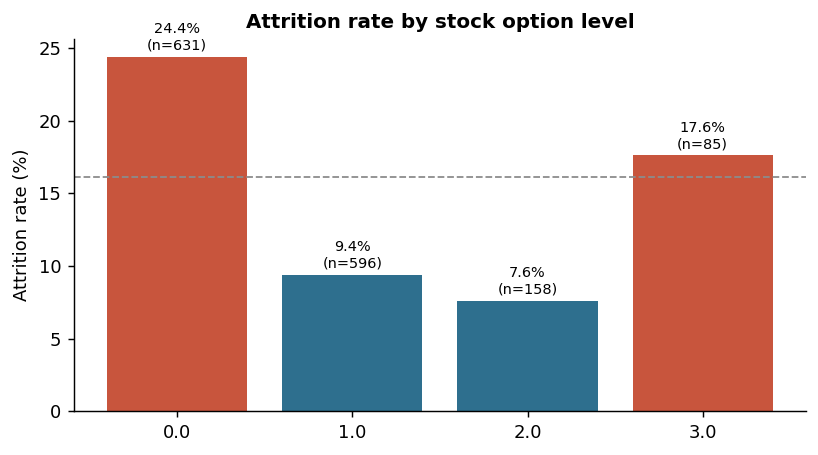
\includegraphics[width=\linewidth]{figures/09_stock.png}\caption{Stock option level}\end{subfigure}
\caption{Attrition by business travel and stock option level}
\label{fig:travelstock}
\end{figure}

\textbf{Satisfaction.} Employees reporting low job satisfaction leave at 22.8\% against 11.3\% for very high satisfaction, and those rating work-life balance as ``bad'' leave at 31.3\%.

\section{Correlation Analysis}

The Pearson correlation matrix was computed with Spark MLlib's \texttt{Correlation.corr} on an assembled feature vector (Figure~\ref{fig:corr}). No single numeric variable correlates strongly with attrition; the largest values are around $-0.17$, for total working years, job level, monthly income, years in current role and age. Attrition is therefore driven by a combination of factors rather than by any one of them, which is why multivariate models are needed. The matrix also shows strong collinearity: monthly income and job level correlate at 0.95, and the tenure variables at 0.5--0.8. Tree models handle this naturally, and regularisation handles it for logistic regression.

\begin{figure}[H]
\centering
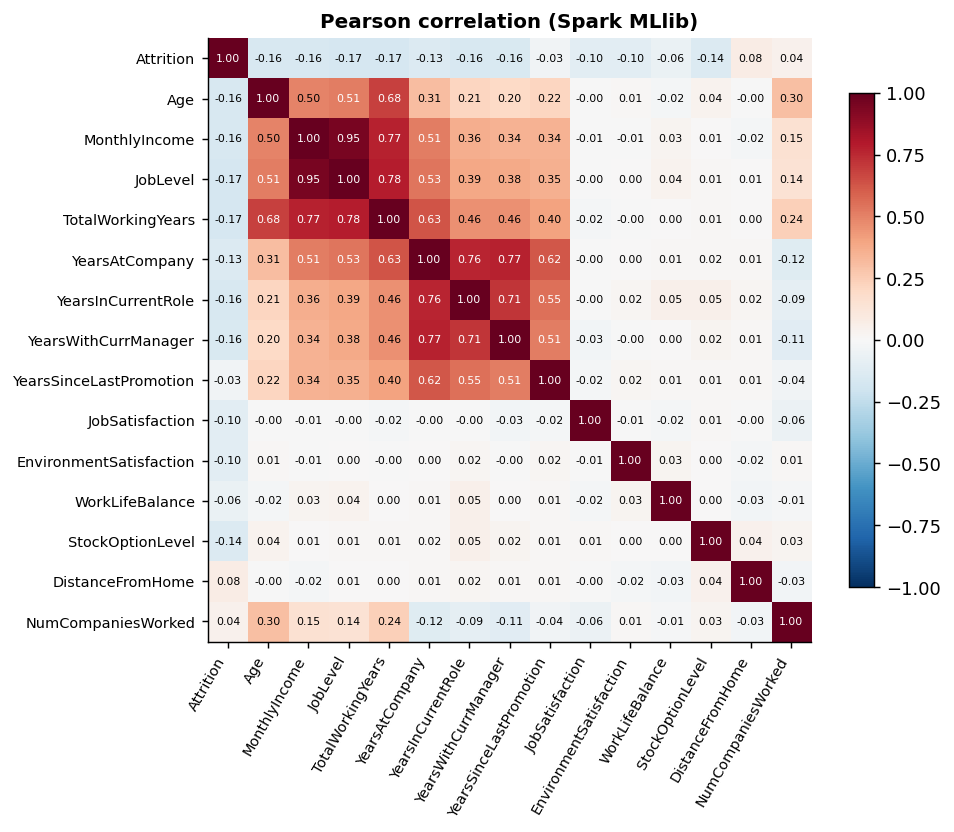
\includegraphics[width=0.82\textwidth]{figures/11_correlation.png}
\caption{Correlation matrix of key numeric variables (Spark MLlib)}
\label{fig:corr}
\end{figure}

\section{Key Findings of the Analysis}

\begin{itemize}
\item The highest-risk profile is a young, single employee in an entry-level role (job level 1), in the first two years at the company, working overtime, with low income and no stock options.
\item Overtime, job role, tenure, income and stock options separate leavers from stayers most clearly.
\item No single variable explains attrition on its own, which justifies a multivariate machine-learning model.
\item Several variables measure the same thing (income, level and experience), so regularisation or tree models are preferred.
\end{itemize}

%================================================
% CHAPTER 4: METHODOLOGY AND SYSTEM DESIGN
%================================================

\chapter{Methodology and System Design}

\section{Overall Methodology}

The project follows the standard data-science life cycle, adapted to Spark (Figure~\ref{fig:method}): understand the business problem, collect the data, explore it with Spark SQL, clean it and engineer features, train and tune models, evaluate and select, deploy, and turn the results into HR actions.

\begin{figure}[H]
\centering
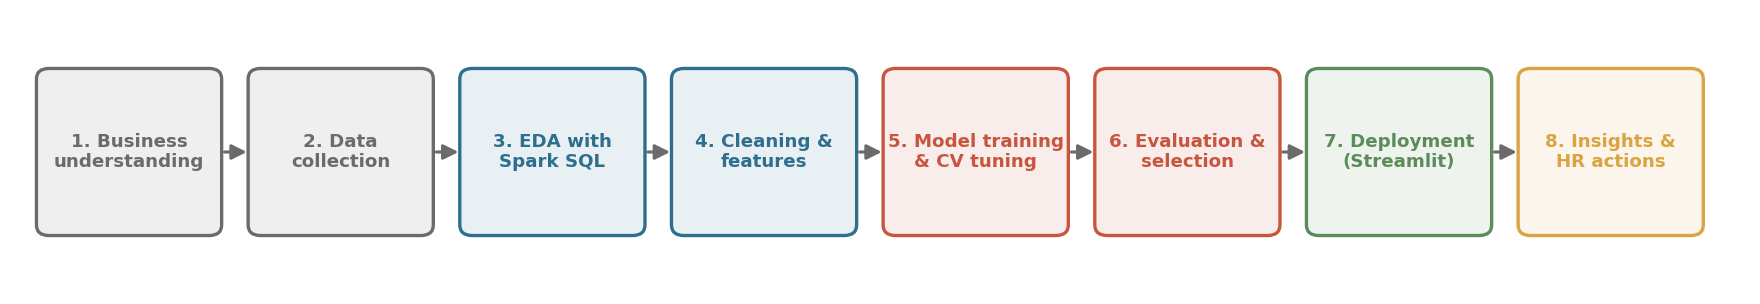
\includegraphics[width=\textwidth]{figures/00_methodology.png}
\caption{Project methodology}
\label{fig:method}
\end{figure}

\section{System Architecture}

Figure~\ref{fig:arch} shows the architecture. The \textbf{data layer} holds the HR dataset and any new records uploaded by users. The \textbf{Spark processing layer} loads, cleans and analyses the data with DataFrames and Spark SQL. The \textbf{Spark MLlib layer} trains and tunes the models and saves the best complete pipeline. The \textbf{model store} keeps the saved model, its metrics and the analysis results. The \textbf{Streamlit application} loads the saved pipeline once and serves the dashboard and predictions to HR users.

\begin{figure}[H]
\centering
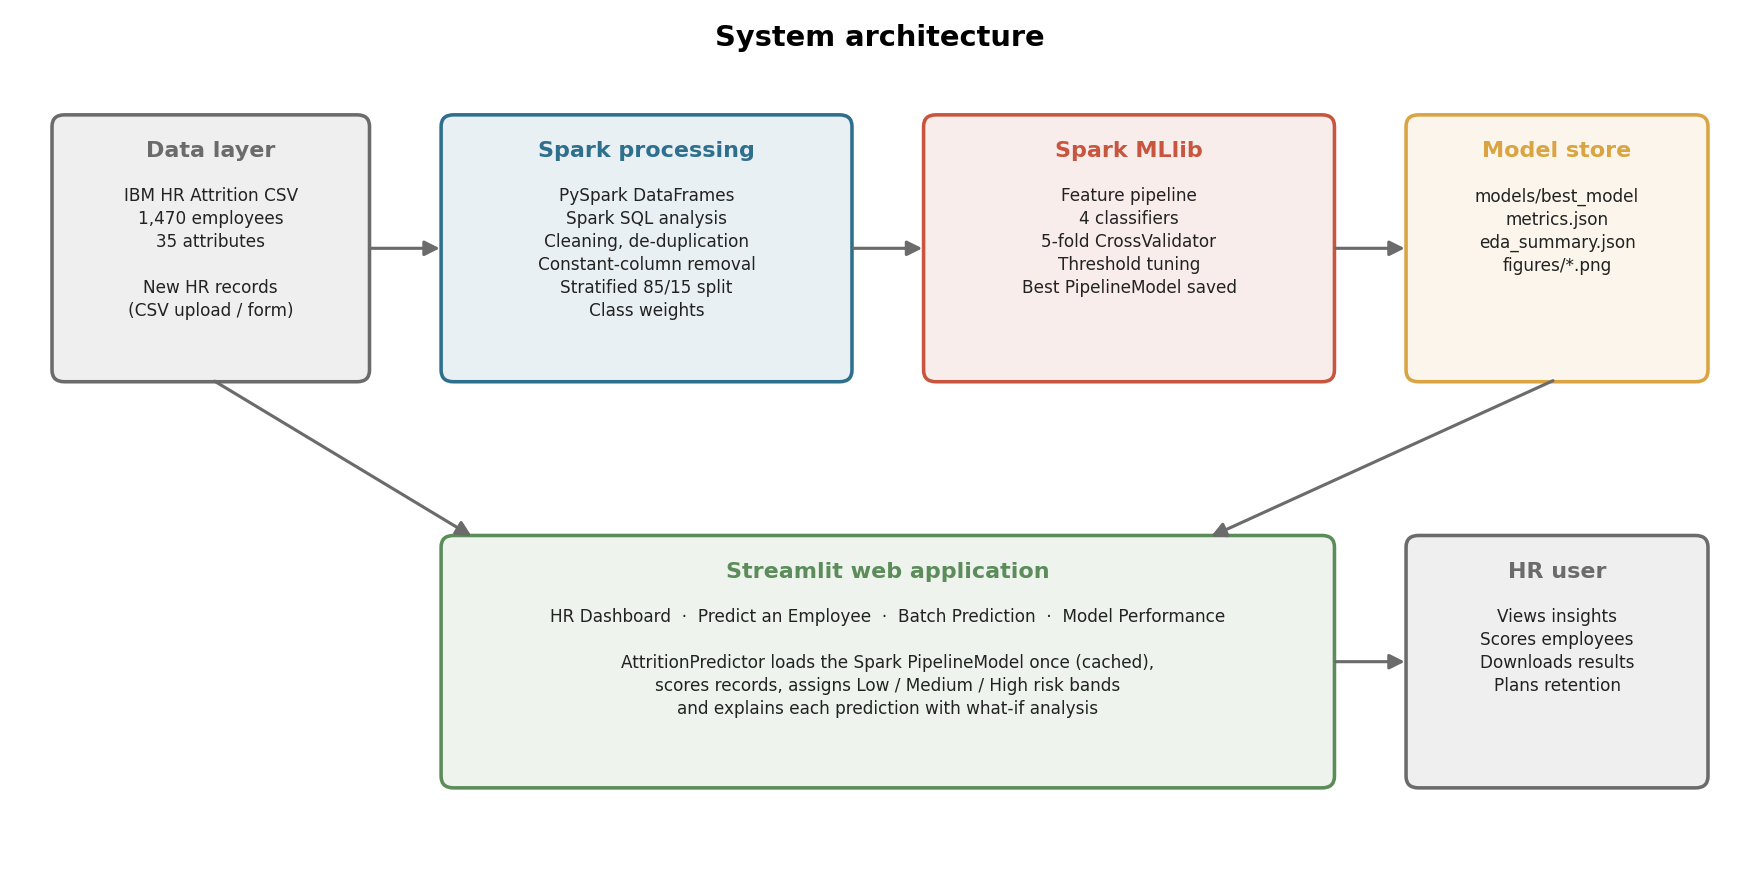
\includegraphics[width=\textwidth]{figures/00_architecture.png}
\caption{System architecture}
\label{fig:arch}
\end{figure}

\section{Feature Engineering}

Five features were derived from the raw attributes to capture relationships the raw columns show only indirectly:

\begin{table}[H]
\centering
\caption{Engineered features}
\label{tab:fe}
\small
\begin{tabularx}{\textwidth}{|P{3.6cm}|P{5.2cm}|L|}
\hline
\textbf{Feature} & \textbf{Formula} & \textbf{Meaning} \\ \hline
IncomePerJobLevel & MonthlyIncome / JobLevel & Pay relative to level: underpaid for the level \\ \hline
TenureRatio & YearsAtCompany / (TotalWorkingYears + 1) & Share of the career spent at this company \\ \hline
YearsPerCompany & TotalWorkingYears / (NumCompaniesWorked + 1) & Average stay per employer: job-hopping tendency \\ \hline
PromotionGap & YearsSinceLastPromotion / (YearsAtCompany + 1) & How stalled the career is at this company \\ \hline
SatisfactionIndex & Mean of five satisfaction / involvement ratings & One overall engagement score \\ \hline
\end{tabularx}
\end{table}

The features are computed by a \texttt{SQLTransformer} stage \emph{inside} the MLlib pipeline. Because of this, the saved model accepts raw HR records directly, and the same formulas are applied identically in training and in the application.

\section{Spark MLlib Pipeline}

Every model shares the same pipeline (Figure~\ref{fig:pipe}):

\begin{enumerate}
\item \textbf{SQLTransformer} adds the five engineered features.
\item \textbf{StringIndexer} converts the seven categorical columns to numeric indices, with the \texttt{keep} option for invalid values, so that an unseen category in new data does not break scoring.
\item \textbf{OneHotEncoder} turns each index into a binary vector, so no false order is implied between categories.
\item \textbf{VectorAssembler} combines the 23 numeric, 5 engineered and encoded categorical features into one vector.
\item \textbf{StandardScaler} centres and scales each feature to mean 0 and standard deviation 1, which logistic regression needs for regularisation to treat features fairly.
\item The \textbf{classifier}.
\end{enumerate}

\begin{figure}[H]
\centering
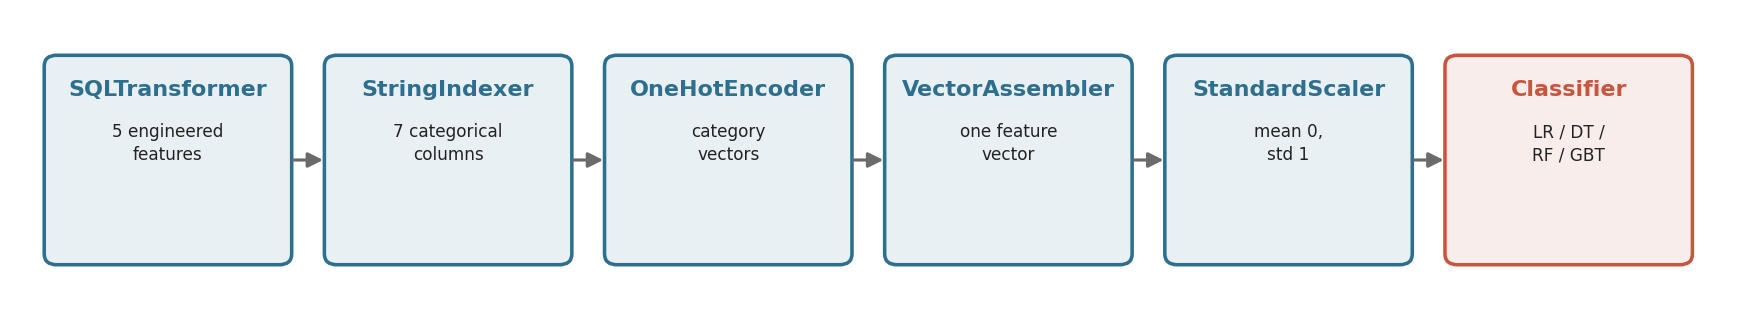
\includegraphics[width=\textwidth]{figures/00_ml_pipeline.png}
\caption{Spark MLlib pipeline}
\label{fig:pipe}
\end{figure}

\section{Data Split}

With only \Leavers{} leavers, the data must be used carefully. It was split into a \textbf{development set (85\%)} and a \textbf{test set (15\%)} stratified on the label so that both parts keep the \AttrRate\% attrition rate. Within each class, employees are ranked by a seeded hash of their employee number and the lowest 15\% go to the test set. Unlike Spark's random \texttt{sampleBy}, whose result depends on how the data happens to be partitioned, this split is exact and identical on every run and every machine, so the reported results can be reproduced. This gave \DevRows{} development employees (\DevLeavers{} leavers) and \TestRowsSplit{} test employees.

\begin{itemize}
\item \textbf{Development set}: hyper-parameter tuning by 5-fold cross-validation, threshold selection from out-of-fold predictions, and model selection.
\item \textbf{Test set}: used once, at the end, for the final reported results. It played no part in any choice, so its results are an unbiased estimate.
\end{itemize}

A three-way split with a separate validation set was tried first. With only about 39 leavers in a 15\% validation set, the threshold and model choice changed noticeably with a few employees, and thresholds tuned on it lowered the F1-score on the test set for every model. Cross-validation uses every development record for both fitting and checking, which gives much more stable choices on a dataset of this size.

\section{Handling Class Imbalance}

Each leaver in the development set was given a weight equal to the ratio of stayers to leavers (about 5.2), and each stayer a weight of 1, through MLlib's \texttt{weightCol} parameter. The two classes therefore contribute equally to the training loss, and the models do not learn to ignore the minority class.

\section{Model Training and Hyper-parameter Tuning}

Each classifier was wrapped in a \texttt{CrossValidator} with a \texttt{ParamGridBuilder} grid, 5 folds, ROC-AUC as the selection metric and a parallelism of 4. Because the whole pipeline is cross-validated, encoders and the scaler are re-fitted inside each fold, so no information leaks from the held-out folds.

\begin{table}[H]
\centering
\caption{Hyper-parameter search grids}
\label{tab:grid}
\small
\begin{tabularx}{\textwidth}{|P{3.6cm}|L|P{1.4cm}|}
\hline
\textbf{Model} & \textbf{Grid searched} & \textbf{Settings} \\ \hline
Logistic Regression & regParam $\in\{0.001, 0.01, 0.1\}$, elasticNetParam $\in\{0, 0.5, 1\}$ & 9 \\ \hline
Decision Tree & maxDepth $\in\{3, 5, 7\}$, minInstancesPerNode $\in\{5, 20\}$ & 6 \\ \hline
Random Forest & numTrees $\in\{100, 200\}$, maxDepth $\in\{5, 8\}$ & 4 \\ \hline
Gradient-Boosted Trees & maxIter $\in\{50, 100\}$, maxDepth $\in\{3, 5\}$ (stepSize 0.1) & 4 \\ \hline
\end{tabularx}
\end{table}

\section{Model Selection and Threshold Tuning}

A classifier outputs a probability of leaving, and a threshold turns it into a yes / no prediction. The default threshold of 0.5 is rarely the best choice for imbalanced data. For each tuned model, the best parameters were re-fitted five times, each time leaving out one fold of the development set, so that every development employee receives an \emph{out-of-fold} (OOF) probability from a model that did not see them in training. The threshold between 0.10 and 0.90 that maximises the F1-score on these out-of-fold predictions was selected. The model with the highest mean cross-validated ROC-AUC was chosen as the final model, and \texttt{CrossValidator} re-fits it on the whole development set.

\section{Evaluation Metrics}

With TP, FP, TN and FN denoting true / false positives and negatives (positive = left):

\begin{align*}
\text{Precision} &= \frac{TP}{TP + FP} & \text{Recall} &= \frac{TP}{TP + FN} \\[4pt]
\text{F1} &= 2\cdot\frac{\text{Precision}\cdot\text{Recall}}{\text{Precision} + \text{Recall}} & \text{Accuracy} &= \frac{TP + TN}{TP + TN + FP + FN}
\end{align*}

\textbf{ROC-AUC} is the probability that the model ranks a randomly chosen leaver above a randomly chosen stayer, and it does not depend on the threshold. \textbf{Recall} matters most to HR, since a missed leaver is a lost employee. \textbf{Precision} matters because every false alarm costs HR time.

\section{Explaining Individual Predictions}

For each prediction the application runs a \textbf{what-if analysis}. For each of 19 factors, such as overtime, income, stock options, satisfaction ratings, travel and tenure, it creates a copy of the employee's record in which only that factor is set to its typical value among employees who stayed (the median for numbers, the most common value for categories). All copies are scored in a single Spark job. The drop in the leave probability shows how much that factor contributes to the employee's risk:

\[
\text{Impact}(f) = P(\text{leave} \mid x) - P(\text{leave} \mid x \text{ with } f \leftarrow \text{typical}_{\text{stayers}}(f))
\]

Factors with a positive impact are listed in order, each with a suggested HR action (for example, ``review workload and overtime'' or ``benchmark pay against the market''). This works with any model, including tree ensembles whose internals are hard to read.

%================================================
% CHAPTER 5: IMPLEMENTATION
%================================================

\chapter{Implementation}

\section{Tools and Technologies}

\begin{table}[H]
\centering
\caption{Tools and technologies used}
\label{tab:tools}
\small
\begin{tabularx}{\textwidth}{|P{3.6cm}|P{3.2cm}|L|}
\hline
\textbf{Layer} & \textbf{Tool} & \textbf{Use in the project} \\ \hline
Language & Python 3.11 & All code \\ \hline
Big-data engine & Apache Spark 3.5 (PySpark) & DataFrames, Spark SQL, local-mode execution \\ \hline
Machine learning & Spark MLlib & Pipeline, transformers, classifiers, CrossValidator \\ \hline
Runtime & Java 17 (Temurin) & JVM required by Spark \\ \hline
Data handling & pandas, NumPy & Small result sets, metric computation \\ \hline
Visualisation & Matplotlib, Plotly & Report charts; interactive app charts \\ \hline
Web application & Streamlit & HR dashboard and prediction interface \\ \hline
Testing & pytest & Automated tests of the pipeline and predictor \\ \hline
Version control & Git, GitHub & Source control and submission \\ \hline
Documentation & \LaTeX{} (Overleaf) & This report \\ \hline
\end{tabularx}
\end{table}

\section{Project Structure}

\begin{lstlisting}
employee-attrition-prediction/
|-- data/            IBM HR dataset + sample file for batch scoring
|-- src/
|   |-- config.py          paths, column lists, feature SQL
|   |-- spark_session.py   local SparkSession (Windows set-up)
|   |-- preprocess.py      load, clean, split, class weights, pipeline
|   |-- eda.py             Spark SQL analysis and charts
|   |-- train.py           training, tuning, selection, evaluation
|   |-- predict.py         scoring, risk bands, what-if explanation, CLI
|   `-- scale_benchmark.py scalability test on enlarged data
|-- app/streamlit_app.py   web application
|-- models/          saved PipelineModel + metrics JSON
|-- reports/figures/ generated charts
|-- tests/           pytest tests
|-- report/          this LaTeX report
`-- ppt/             presentation
\end{lstlisting}

\section{Module Description}

\textbf{config.py} holds every constant in one place: file paths, the lists of numeric and categorical columns, the SQL for the engineered features and the allowed values for the application's inputs.

\textbf{preprocess.py} loads the CSV into Spark, removes the constant columns, adds the numeric label, performs the reproducible, hash-based stratified development / test split, adds class weights and builds the feature stages of the pipeline.

\textbf{eda.py} registers the cleaned data as a Spark SQL view, computes attrition rates by each factor and band with SQL, computes the correlation matrix with MLlib and saves the charts and a JSON summary.

\textbf{train.py} runs the cross-validated grid search for each of the four models, tunes the threshold on out-of-fold predictions, evaluates on test data, saves the best \texttt{PipelineModel} with Spark's model writer and draws the ROC, precision--recall, comparison, confusion-matrix and feature-importance charts.

\textbf{predict.py} contains the \texttt{AttritionPredictor} class used by the application. It loads the saved pipeline, converts incoming pandas records to a Spark DataFrame with a fixed schema, returns the probability, a risk band (High at or above the tuned threshold, Medium at or above 60\% of it, Low otherwise) and the predicted label, and produces the what-if explanation. It can also be run from the command line to score a CSV file.

The core of the training step for one model is:

\begin{lstlisting}[language=Python]
pipeline = Pipeline(stages=feature_stages() + [classifier])
cv = CrossValidator(estimator=pipeline, estimatorParamMaps=grid,
                    evaluator=BinaryClassificationEvaluator(metricName="areaUnderROC"),
                    numFolds=5, parallelism=4, seed=42)
best = cv.fit(dev).bestModel                        # tuned on development data only
threshold = best_threshold(*oof_scores(clf, params, dev))  # out-of-fold predictions
test_metrics = metrics_at(*scores(best, test), threshold)   # reported once
best.write().overwrite().save("models/best_model")
\end{lstlisting}

\section{Web Application}

The Streamlit application has five pages, listed in a sidebar that also shows the model in use and its test AUC:

\begin{enumerate}
\item \textbf{HR Dashboard}: key figures (headcount, leavers, attrition rate, average income) and interactive charts of attrition by overtime, job role, tenure, income, marital status and age. Department, gender and overtime filters update every chart.
\item \textbf{Predict an Employee}: a form grouped into Personal, Job, Compensation, Satisfaction and Tenure sections, with rating scales shown in words (``Low'', ``Very High''). The result shows a gauge of the leave probability against the threshold, the risk band, and a table of the top risk drivers with suggested HR actions. Inputs are checked for consistency, for example that years at the company do not exceed total working years.
\item \textbf{Batch Prediction}: upload a CSV of employee records, or use the bundled sample. The file is validated, every employee is scored with Spark, and the page shows the counts by risk band, a risk-band chart, the average risk by department and a ranked table, with the results available for download.
\item \textbf{Model Performance}: the comparison of all four models, the ROC curve, the confusion matrix and the feature importance of the selected model.
\item \textbf{About}: a summary of the project and the method.
\end{enumerate}

The Spark session and model are loaded once and cached with \texttt{st.cache\_resource}, so later predictions return in about a second.

\section{Testing}

Automated tests (\texttt{pytest}) check that cleaning keeps all 1,470 records and removes the constant columns, that the three-way split is disjoint, covers every record and preserves the attrition rate, that the predictor scores the sample file with valid probabilities and risk bands, and that missing columns in an uploaded file are reported. The application was also tested by hand with typical, high-risk and inconsistent inputs and with valid and invalid CSV files.

\section{Source Code Repository}

The complete project, including code, data, the trained model, charts, tests, this report and the presentation, is published on GitHub at:

\begin{center}
\url{https://github.com/varunmundhada/employee-attrition-prediction}
\end{center}

The README gives one-command set-up and run instructions (Appendix~\ref{app:run}).

%================================================
% CHAPTER 6: RESULTS AND DISCUSSION
%================================================

\chapter{Results and Discussion}

\section{Model Comparison}

Table~\ref{tab:results} compares the four tuned models. CV AUC is the mean over the five folds and was used for model selection; OOF AUC is computed on the out-of-fold predictions used for the threshold. All other columns are on the untouched test set of \TestRowsSplit{} employees, at each model's tuned threshold.

\begin{table}[H]
\centering
\caption{Model comparison (test-set metrics at the tuned threshold; best model in bold)}
\label{tab:results}
\footnotesize
\setlength{\tabcolsep}{4pt}
\begin{tabular}{|p{3.3cm}|c|c|c|c|c|c|c|c|}
\hline
\textbf{Model} & \textbf{CV AUC} & \textbf{OOF AUC} & \textbf{Test AUC} & \textbf{Acc.} & \textbf{Prec.} & \textbf{Recall} & \textbf{F1} & \textbf{Thr.} \\ \hline
\tabinput{generated/model_table.tex}
\end{tabular}
\end{table}

\begin{table}[H]
\centering
\caption{Selected hyper-parameters and training time (grid search with 5-fold CV)}
\label{tab:params}
\small
\begin{tabularx}{\textwidth}{|P{4cm}|L|P{2.2cm}|}
\hline
\textbf{Model} & \textbf{Best parameters} & \textbf{Time (s)} \\ \hline
\tabinput{generated/params_table.tex}
\end{tabularx}
\end{table}

\begin{figure}[H]
\centering
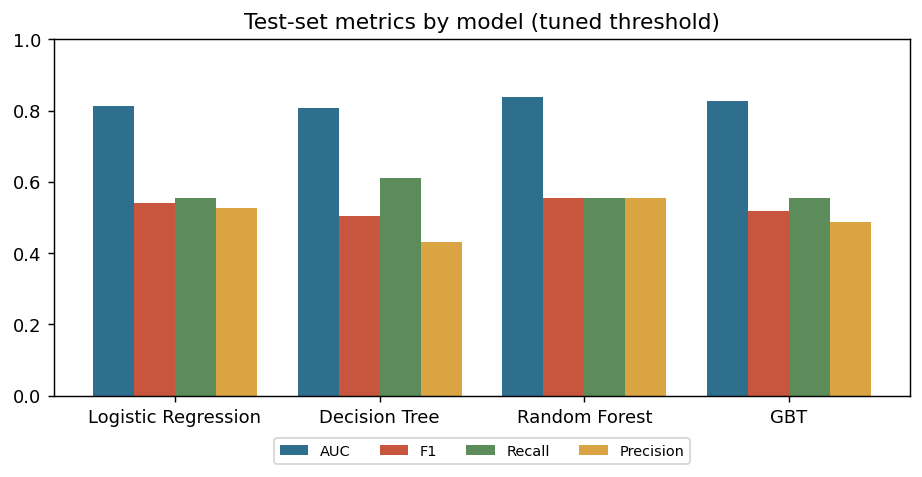
\includegraphics[width=0.85\textwidth]{figures/14_model_comparison.png}
\caption{Test-set metrics by model}
\label{fig:compare}
\end{figure}

\textbf{\BestModel} was selected, with a cross-validated AUC of \BestCVAUC{} and a test AUC of \textbf{\BestTestAUC}. On the test set it reached an accuracy of \BestAcc\%, a precision of \BestPrec\%, a recall of \BestRecall\% and an F1-score of \BestFone\% at a threshold of \BestThr. The ROC and precision--recall curves (Figure~\ref{fig:curves}) show that every model ranks employees far better than chance. On this small, mostly linear dataset the regularised logistic regression matches or beats the tree ensembles in cross-validation, in line with Zhao et al. \cite{zhao2019employee}, and it has the added advantage that its coefficients can be read directly. The single decision tree is clearly the weakest, as expected.

The test AUC (\BestTestAUC) is lower than the cross-validated AUC (\BestCVAUC). With only \TestLeavers{} leavers in the test set, a handful of employees can move the AUC by several points: during development, runs with different random splits gave test AUCs anywhere between 0.79 and 0.87 for the same models. The cross-validated figure, averaged over five folds of \DevRows{} employees, is the more stable estimate of performance on new data, and the test figure is a conservative check that the model was not over-tuned.

\begin{figure}[H]
\centering
\begin{subfigure}{0.49\textwidth}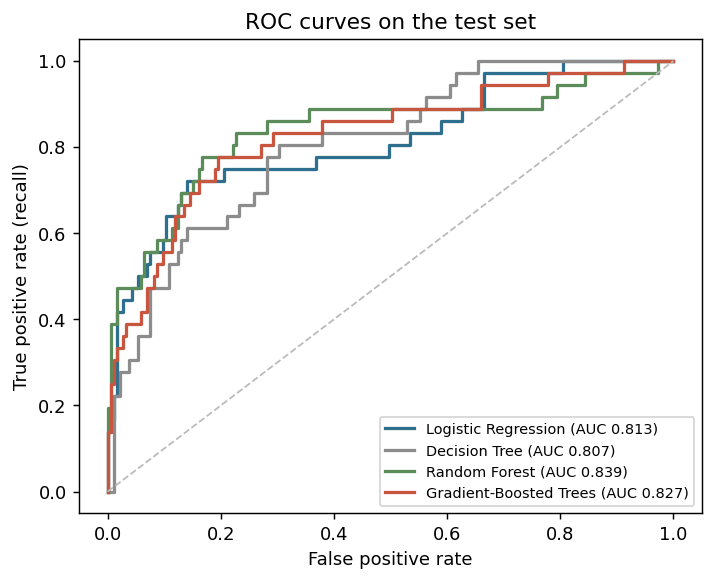
\includegraphics[width=\linewidth]{figures/12_roc_curves.png}\caption{ROC curves}\end{subfigure}
\begin{subfigure}{0.49\textwidth}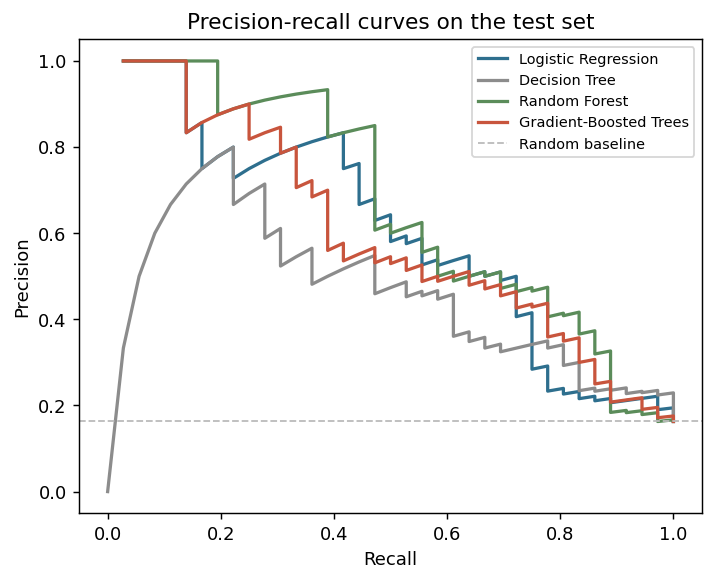
\includegraphics[width=\linewidth]{figures/13_pr_curves.png}\caption{Precision--recall curves}\end{subfigure}
\caption{ROC and precision--recall curves on the test set}
\label{fig:curves}
\end{figure}

\section{Effect of Threshold Tuning}

Table~\ref{tab:thr} compares each model at the default threshold of 0.5 with the threshold tuned on the out-of-fold predictions. Because class weights already rebalance the training, all thresholds stay near the middle of the range, and tuning changes F1 only slightly. What tuning really changes is the balance between precision and recall. For the selected model, the F1-optimal threshold of \BestThr{} finds \BestRecall\% of the leavers with a precision of \BestPrec\%, while the default of 0.5 finds \BestRecallHalf\% of them but with a precision of only \BestPrecHalf\%. The threshold is therefore a business choice: an HR team that can hold many stay interviews should use a lower threshold to catch more leavers, and a team with limited capacity a higher one. The application shows the threshold on the risk gauge, and the Medium risk band covers employees just below it.

\begin{table}[H]
\centering
\caption{Default (0.5) versus tuned threshold on the test set}
\label{tab:thr}
\small
\begin{tabular}{|p{3.6cm}|c|c|c|c|c|c|}
\hline
 & \multicolumn{3}{c|}{\textbf{Threshold 0.5}} & \multicolumn{3}{c|}{\textbf{Tuned threshold}} \\ \hline
\textbf{Model} & \textbf{Prec.} & \textbf{Recall} & \textbf{F1} & \textbf{Thr.} & \textbf{Recall} & \textbf{F1} \\ \hline
\tabinput{generated/threshold_table.tex}
\end{tabular}
\end{table}

\section{Confusion Matrix}

Of the \TestLeavers{} employees in the test set who actually left, the selected model correctly flagged \CmTP{} and missed \CmFN{}. Of the employees who stayed, it raised \CmFP{} false alarms and correctly cleared \CmTN{} (Figure~\ref{fig:cm}). For HR, a list of flagged employees in which a substantial share are true leavers is a far better use of retention effort than reviewing everyone.

\begin{figure}[H]
\centering
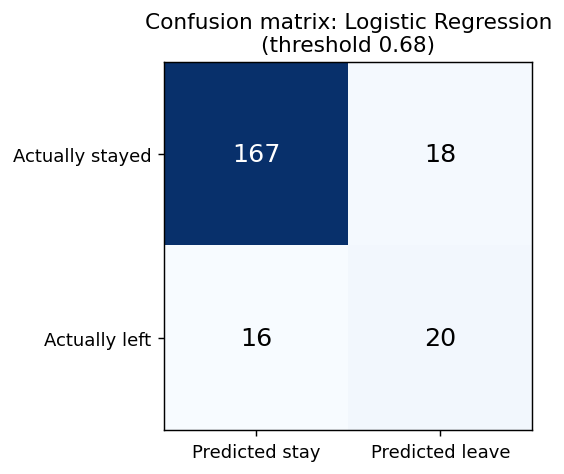
\includegraphics[width=0.5\textwidth]{figures/15_confusion_matrix.png}
\caption{Confusion matrix of the selected model on the test set}
\label{fig:cm}
\end{figure}

\section{Feature Importance}

Figure~\ref{fig:imp} and Table~\ref{tab:imp} list the most influential features of the selected model; the top feature is \textbf{\TopFeature}. Because the selected model is a logistic regression on standardised features, each bar is a coefficient. A red bar (positive) raises the odds of leaving, and a blue bar (negative) lowers them, and the bar lengths can be compared directly. The ranking agrees with the exploratory analysis and with the literature \cite{fallucchi2020predicting}. A long time since the last promotion, working overtime, frequent business travel, many previous employers, a long commute and being single raise the risk. A high overall satisfaction index, a long relationship with the current manager, more years in the current role, higher environment satisfaction and more training lower it. Overtime appears twice (\texttt{Yes} and \texttt{No}) because each category has its own one-hot slot; the two coefficients are mirror images. The engineered \texttt{SatisfactionIndex} is the second-strongest feature, which supports the feature-engineering step. Most of these factors (promotion, overtime, travel, satisfaction, manager relationship, training) are \emph{actionable}, so HR can act on them directly.

\begin{figure}[H]
\centering
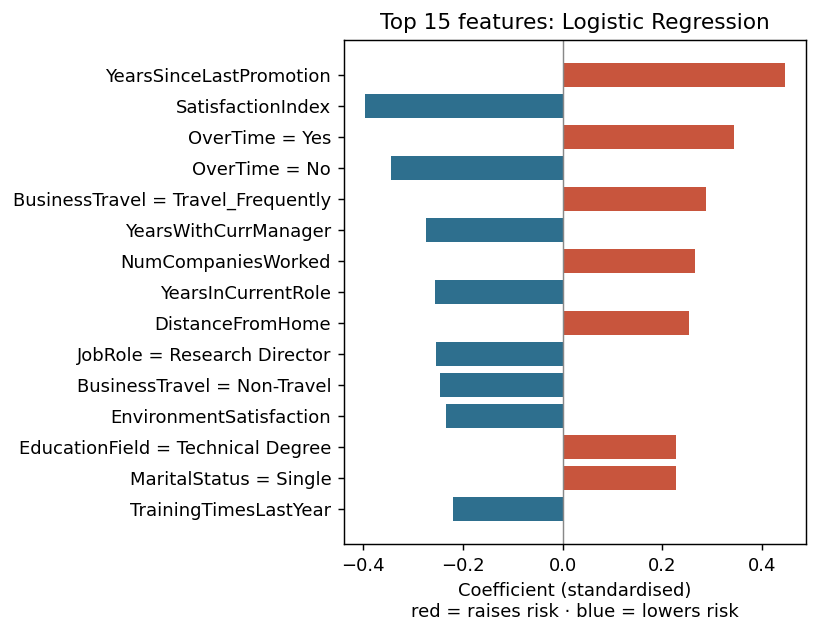
\includegraphics[width=0.78\textwidth]{figures/16_feature_importance.png}
\caption{Top 15 features of the selected model}
\label{fig:imp}
\end{figure}

\begin{table}[H]
\centering
\caption{Top 10 features of the selected model}
\label{tab:imp}
\small
\begin{tabular}{|c|p{7cm}|c|}
\hline
\textbf{Rank} & \textbf{Feature} & \textbf{Importance} \\ \hline
\tabinput{generated/importance_table.tex}
\end{tabular}
\end{table}

\section{Scalability on Larger Data}

To show that the solution is a big-data pipeline and not only a small-data model, the dataset was enlarged synthetically: each record was copied up to 500 times, with $\pm 5\%$ random noise on nine numeric columns, to reach about 735,000 records. The same Spark pipeline was trained on each size with fixed parameters (Table~\ref{tab:scale}, Figure~\ref{fig:scale}). The code did not change at any size. Training time grows much more slowly than the data. Going from 14,700 to 735,000 rows (50 times more data), logistic-regression training went from about 12 to 27 seconds and random-forest training from about 9 to 54 seconds on one laptop, because Spark spreads the work over all processor cores. On a cluster the same code would spread across machines. The first, smallest run is slower than the second because it includes Spark's start-up and JVM warm-up.

\begin{table}[H]
\centering
\caption{Training and scoring time as the data grows (Spark local mode, one laptop)}
\label{tab:scale}
\small
\begin{tabular}{|r|l|c|c|c|}
\hline
\textbf{Rows} & \textbf{Model} & \textbf{Fit (s)} & \textbf{Score (s)} & \textbf{AUC} \\ \hline
\tabinput{generated/scale_table.tex}
\end{tabular}
\end{table}

\IfFileExists{figures/17_scalability.png}{%
\begin{figure}[H]
\centering
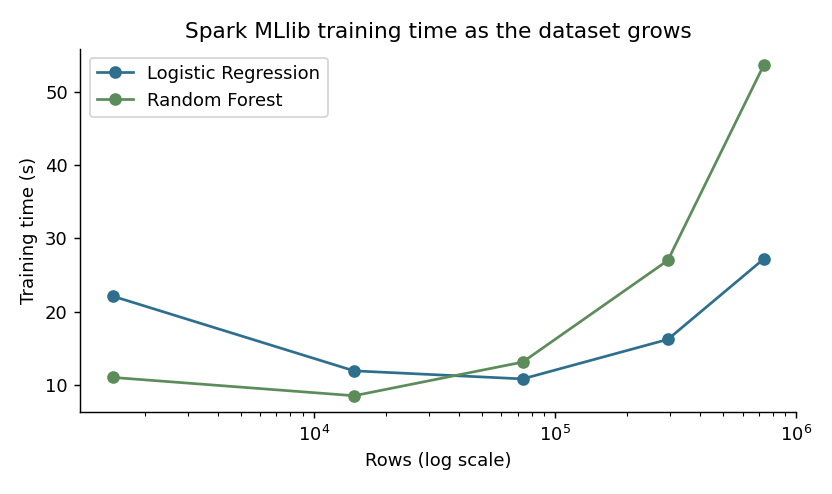
\includegraphics[width=0.7\textwidth]{figures/17_scalability.png}
\caption{Training time versus data size}
\label{fig:scale}
\end{figure}}{}

The AUC on the enlarged data is higher than on the original data because copies of the same employee can fall in both the training and the test part, so these AUC values measure the pipeline's behaviour at scale, not its accuracy. The accuracy results are those in Table~\ref{tab:results}.

\section{Business Insights and Recommendations}

\begin{table}[H]
\centering
\caption{Findings and recommended HR actions}
\label{tab:actions}
\small
\begin{tabularx}{\textwidth}{|P{5.2cm}|L|}
\hline
\textbf{Finding} & \textbf{Recommended action} \\ \hline
Overtime workers leave at \OTYes\% vs \OTNo\% & Monitor overtime hours; rebalance workload or add headcount in teams with sustained overtime \\ \hline
Highest risk in the first two years (34.9\%) & Structured onboarding, buddy programme and 30/60/90-day check-ins \\ \hline
Low income and job level 1 roles at highest risk & Benchmark entry-level pay; publish clear progression paths from level 1 \\ \hline
No stock options: 24.4\% attrition & Extend stock options or retention bonuses to high performers at level 0 \\ \hline
Frequent travel: 24.9\% attrition & Rotate travel duties; offer travel allowances or remote alternatives \\ \hline
Low satisfaction and poor work-life balance & Regular pulse surveys; stay interviews for low scorers; flexible hours \\ \hline
\TopRole s at \TopRoleRate\% & Targeted retention plan for the sales-representative role (incentives, coaching) \\ \hline
\end{tabularx}
\end{table}

\section{Limitations}

\begin{itemize}
\item The dataset is synthetic, created by IBM, and has only 1,470 records, so the test set is small and the metrics carry some uncertainty.
\item Each record is a snapshot; the model does not see how an employee's situation changed over time.
\item The what-if explanation changes one factor at a time and does not capture interactions between factors.
\item The model learns from past decisions and could carry their biases. Protected attributes such as gender and age must be reviewed before use on real data.
\end{itemize}

%================================================
% CHAPTER 7: CONCLUSION AND FUTURE SCOPE
%================================================

\chapter{Conclusion and Future Scope}

\section{Conclusion}

This project built a complete, working employee attrition prediction system on Apache Spark. Exploratory analysis with Spark SQL showed that attrition concentrates among young, early-career, lower-paid employees, especially those working overtime, travelling frequently, without stock options and with low satisfaction. A Spark MLlib pipeline with five engineered features was used to train and tune four classifiers by cross-validation, with class weights for the imbalanced target. Selecting the model and threshold on the development data alone kept the final test evaluation unbiased.

The selected model, \BestModel, achieved a test ROC-AUC of \BestTestAUC{} and found \BestRecall\% of the employees who left. The model is deployed in a Streamlit application that gives HR a dashboard, individual risk predictions with explanations and suggested actions, and batch scoring. A scalability test showed the pipeline running unchanged on about 735,000 records. All objectives set in Chapter 1 were met.

\begin{table}[H]
\centering
\caption{Objectives versus achievement}
\label{tab:obj}
\small
\begin{tabularx}{\textwidth}{|P{6.2cm}|L|}
\hline
\textbf{Objective} & \textbf{Achieved} \\ \hline
Analyse attrition factors with Spark & Spark SQL analysis of 12 factors and an MLlib correlation matrix (Chapter 3) \\ \hline
Reusable Spark MLlib pipeline & Six-stage pipeline with in-pipeline feature engineering (Section 4.4) \\ \hline
Train and compare four classifiers & LR, DT, RF and GBT tuned with 5-fold CV (Table~\ref{tab:results}) \\ \hline
Unbiased selection and evaluation & 85/15 stratified split; CV and out-of-fold tuning; test used once \\ \hline
Explain predictions & What-if analysis with suggested HR actions (Section 4.9) \\ \hline
Working application and scalability & Streamlit application (Chapter 5); test up to about 735k rows (Section 6.5) \\ \hline
\end{tabularx}
\end{table}

\section{Future Scope}

\begin{itemize}
\item \textbf{Real HR data and time series}: train on an organisation's own records, adding monthly snapshots so the model sees trends such as falling satisfaction or rising overtime.
\item \textbf{More data sources}: attendance, leave, engagement surveys and performance reviews, joined in Spark, following the ``big data to deep data'' direction of Yahia et al. \cite{yahia2021big}.
\item \textbf{Cluster deployment and scheduling}: run the pipeline on a Spark cluster (for example Databricks or Amazon EMR) with monthly retraining and drift monitoring.
\item \textbf{Richer explanations}: SHAP values to capture interactions between factors.
\item \textbf{Fairness auditing}: check prediction rates across gender and age groups before any real use.
\item \textbf{Survival analysis}: predict \emph{when} an employee is likely to leave, not only whether.
\end{itemize}

%================================================
% REFERENCES
%================================================

\renewcommand{\bibname}{References}
\nocite{spark_docs, streamlit_docs}
\bibliographystyle{IEEEtran}
\bibliography{references}

%================================================
% APPENDICES
%================================================

\appendix

\chapter{Application Screenshots}

\IfFileExists{figures/app_01_dashboard.png}{%
\begin{figure}[H]
\centering
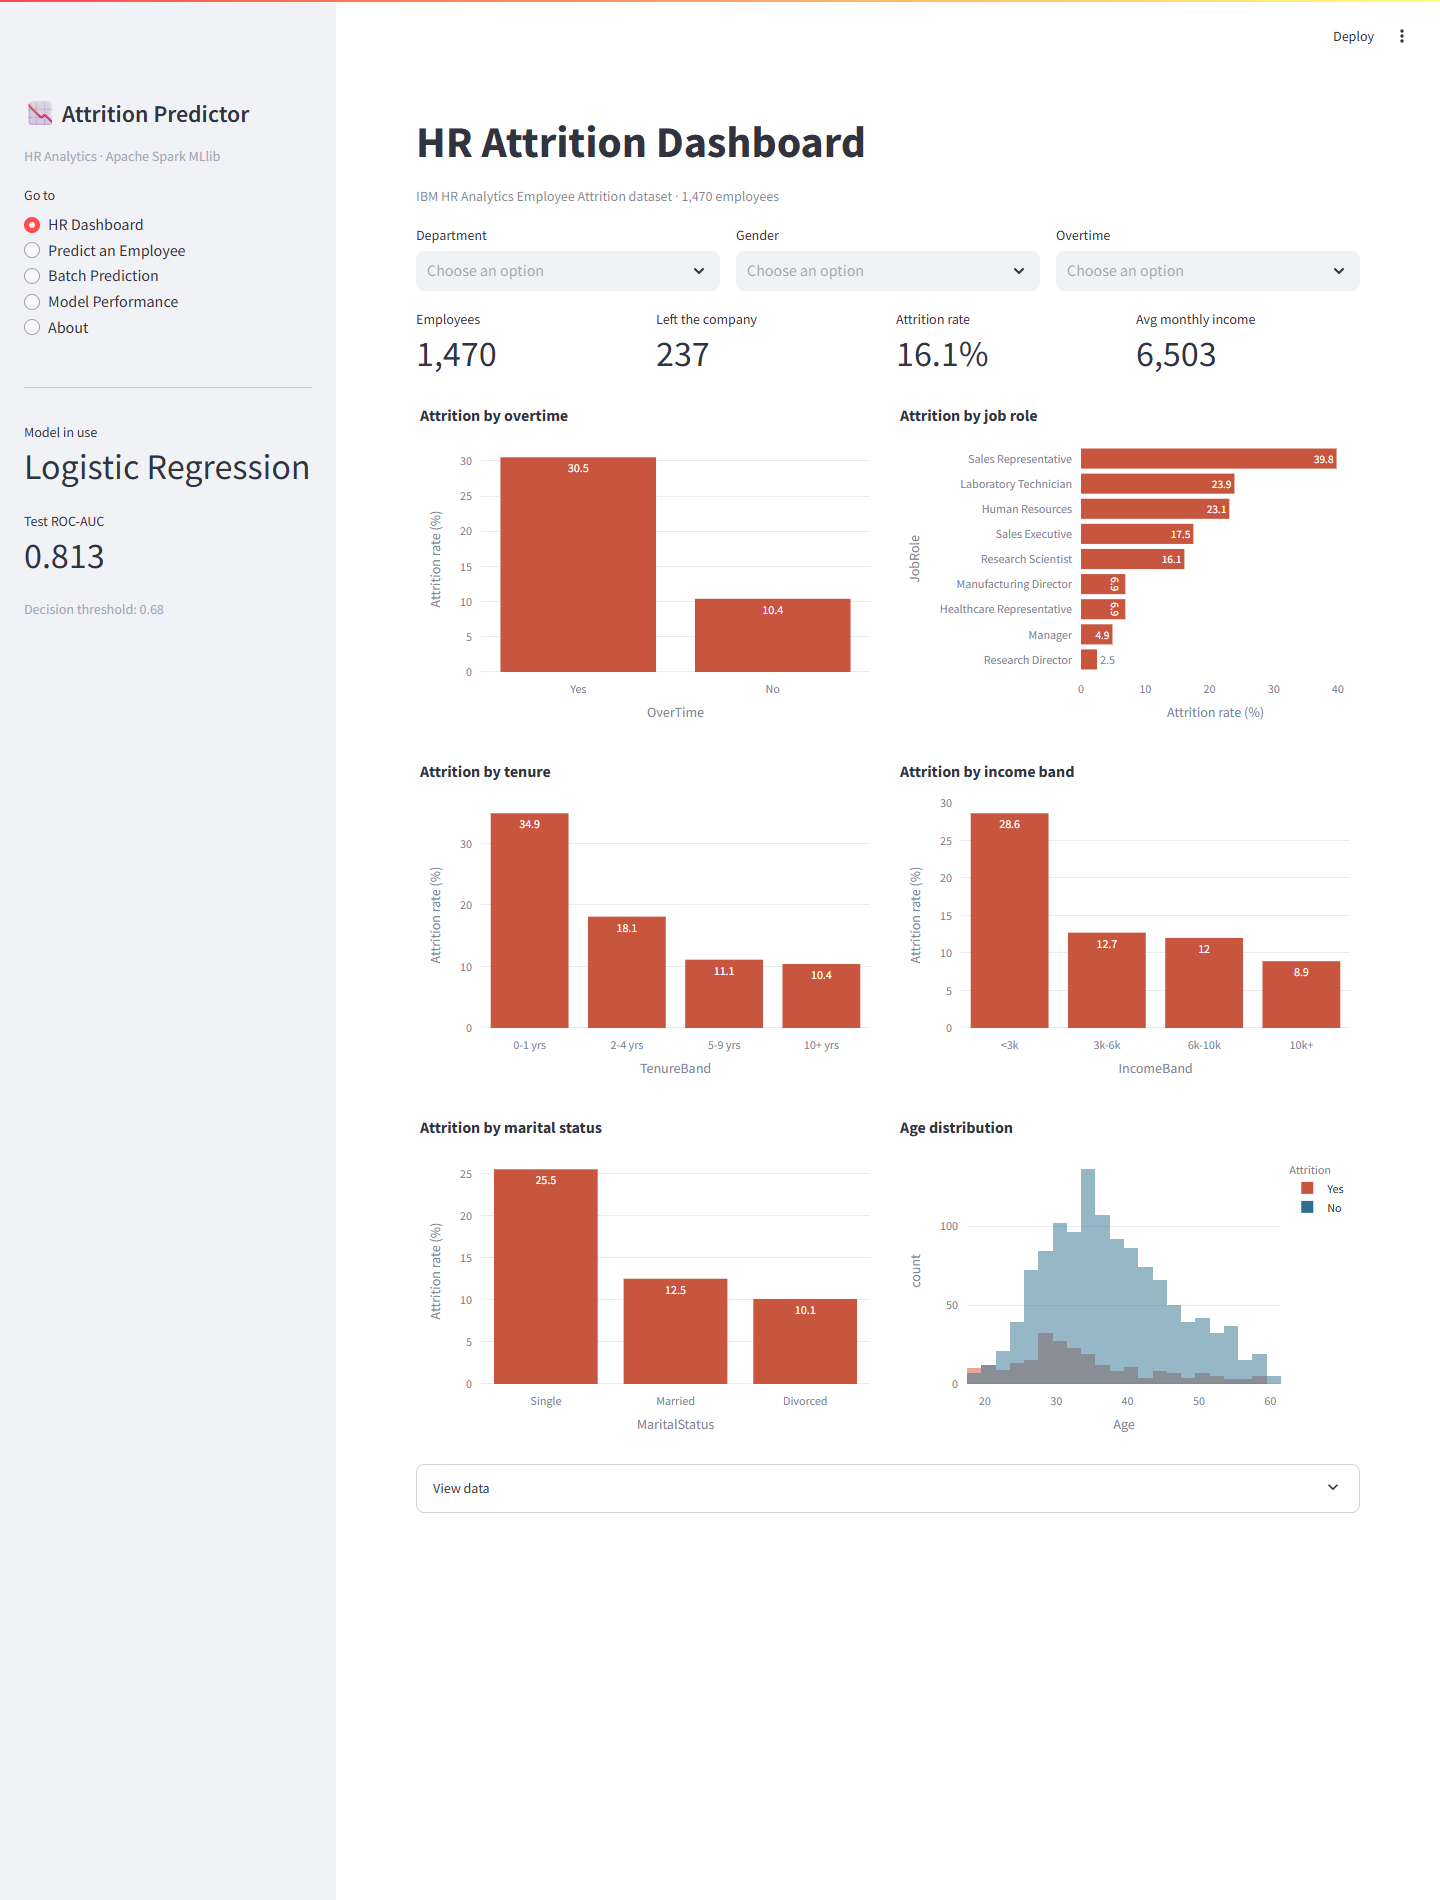
\includegraphics[width=\textwidth,height=0.75\textheight,keepaspectratio]{figures/app_01_dashboard.png}
\caption{HR Dashboard page}
\end{figure}}{}

\IfFileExists{figures/app_02_predict_form.png}{%
\begin{figure}[H]
\centering
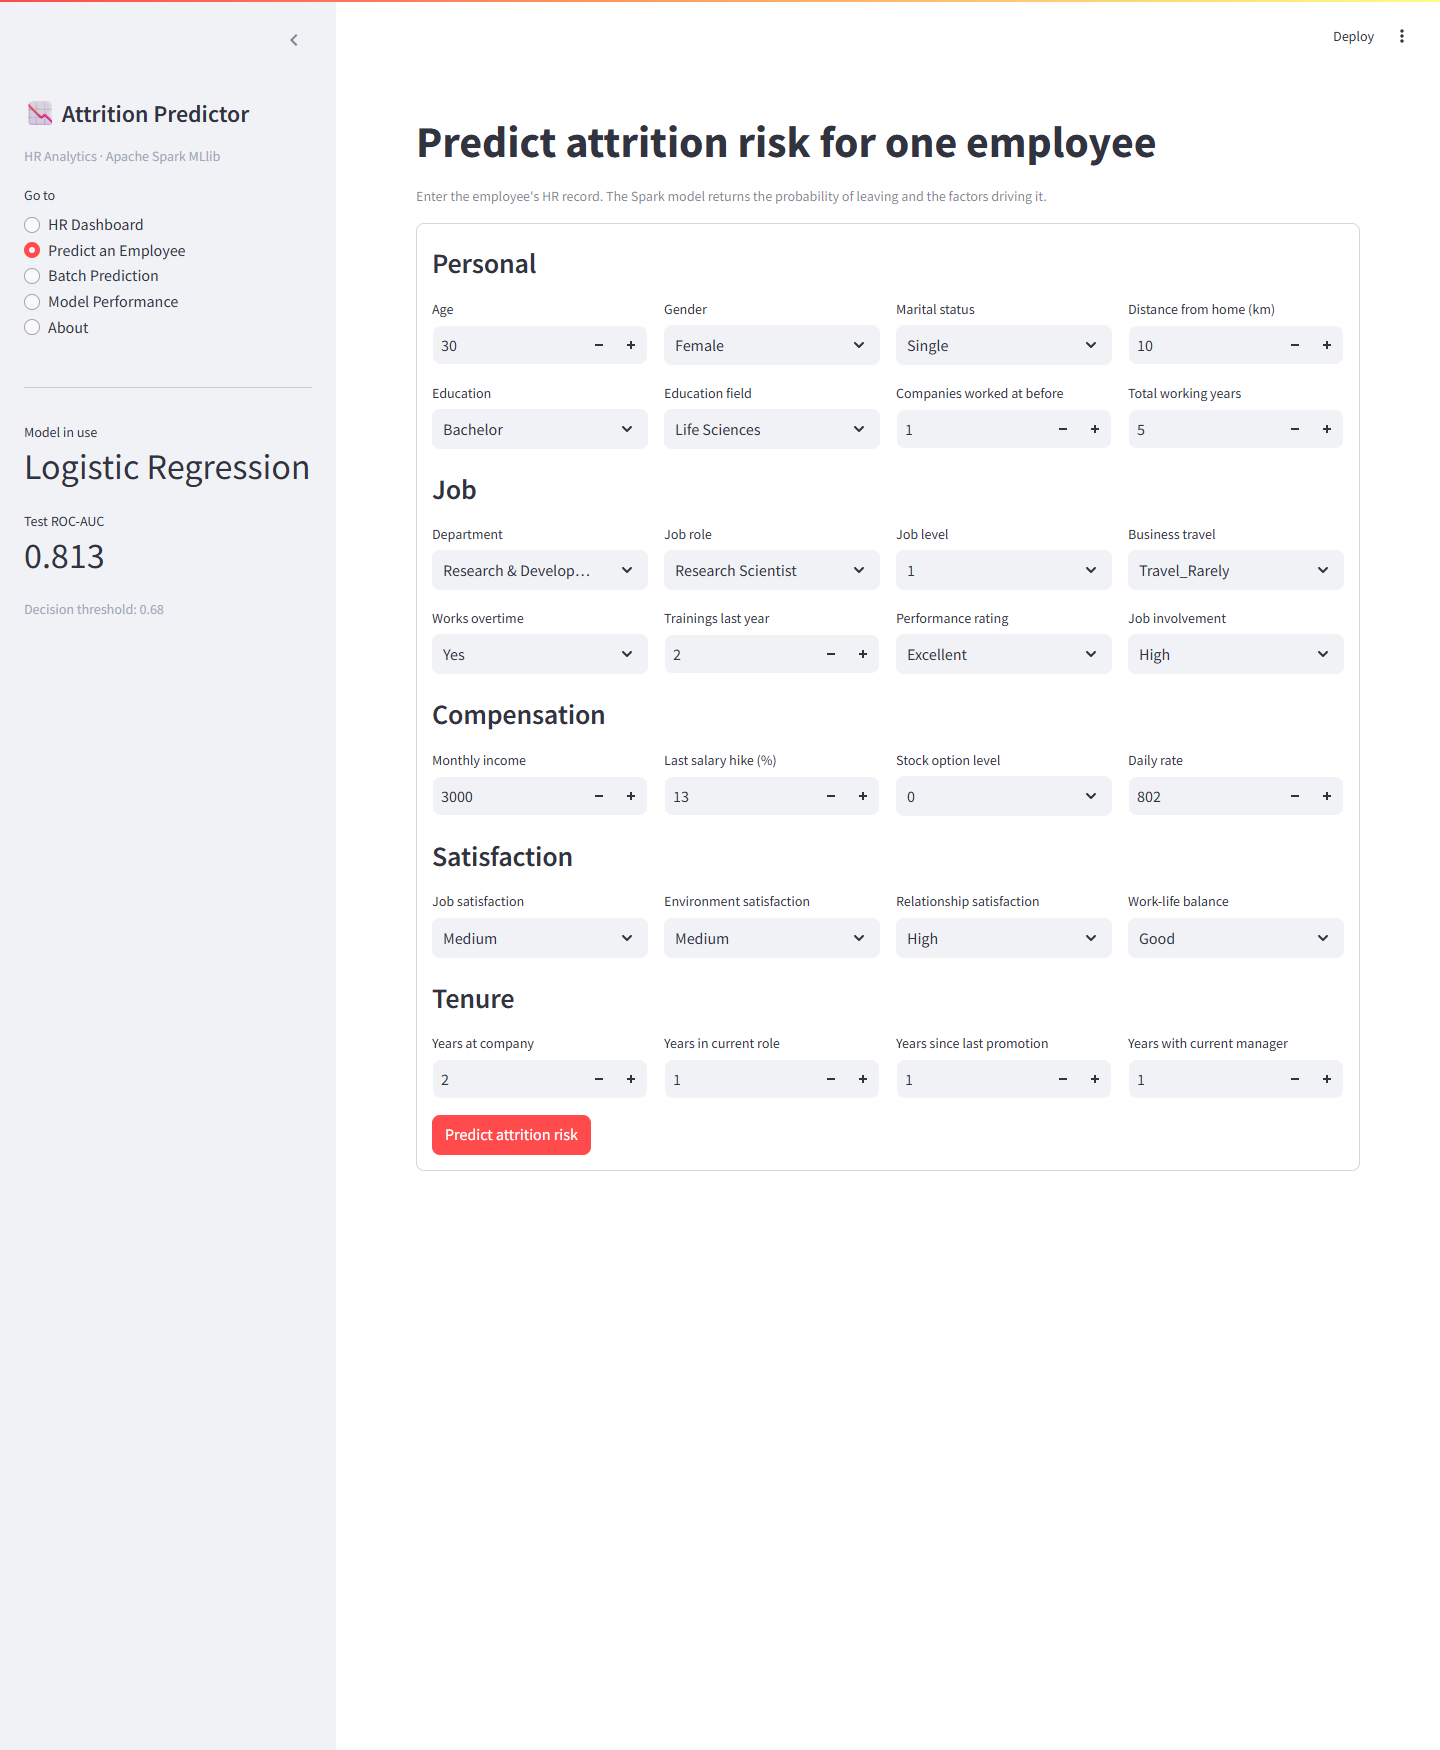
\includegraphics[width=\textwidth,height=0.75\textheight,keepaspectratio]{figures/app_02_predict_form.png}
\caption{Predict an Employee: input form}
\end{figure}}{}

\IfFileExists{figures/app_03_predict_result.png}{%
\begin{figure}[H]
\centering
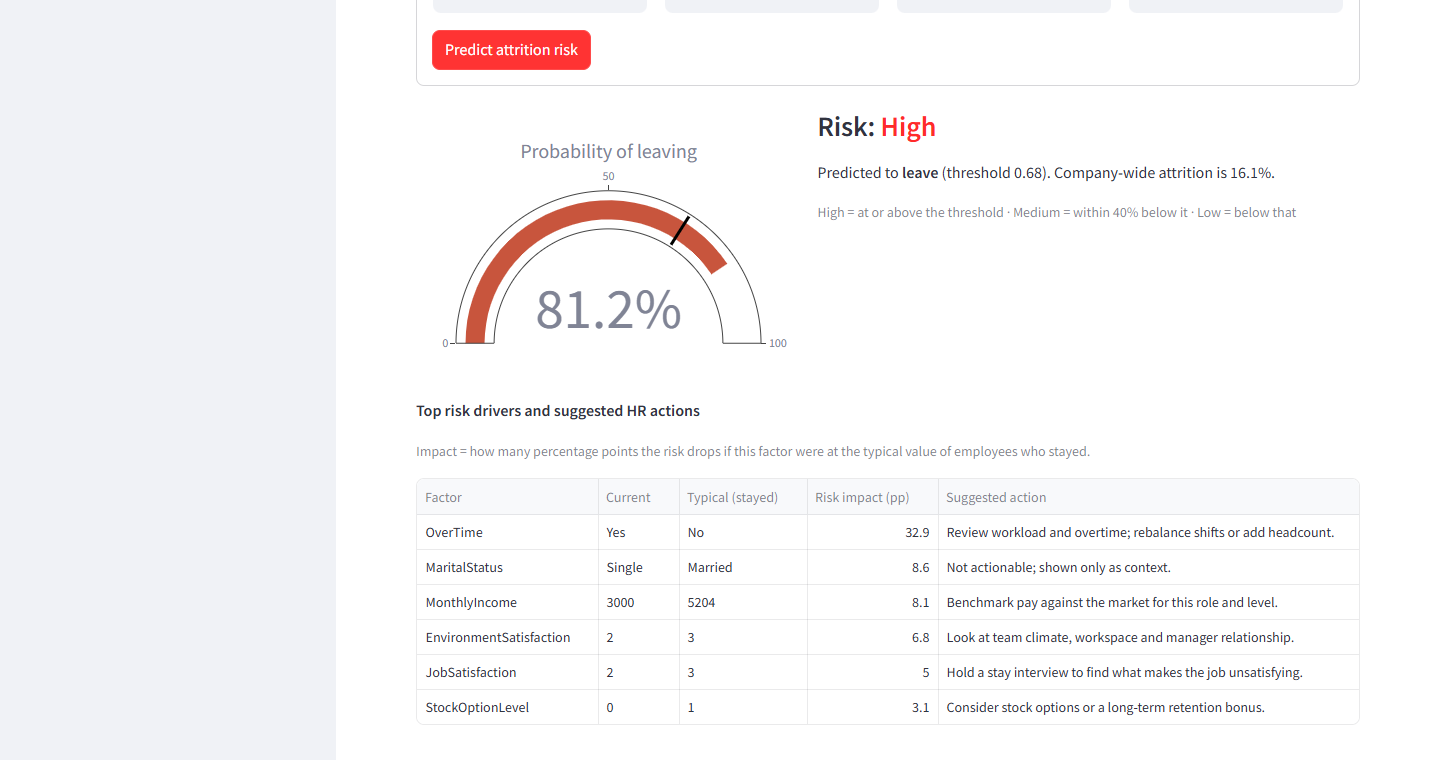
\includegraphics[width=\textwidth,height=0.75\textheight,keepaspectratio]{figures/app_03_predict_result.png}
\caption{Predict an Employee: risk gauge, drivers and suggested actions}
\end{figure}}{}

\IfFileExists{figures/app_04_batch.png}{%
\begin{figure}[H]
\centering
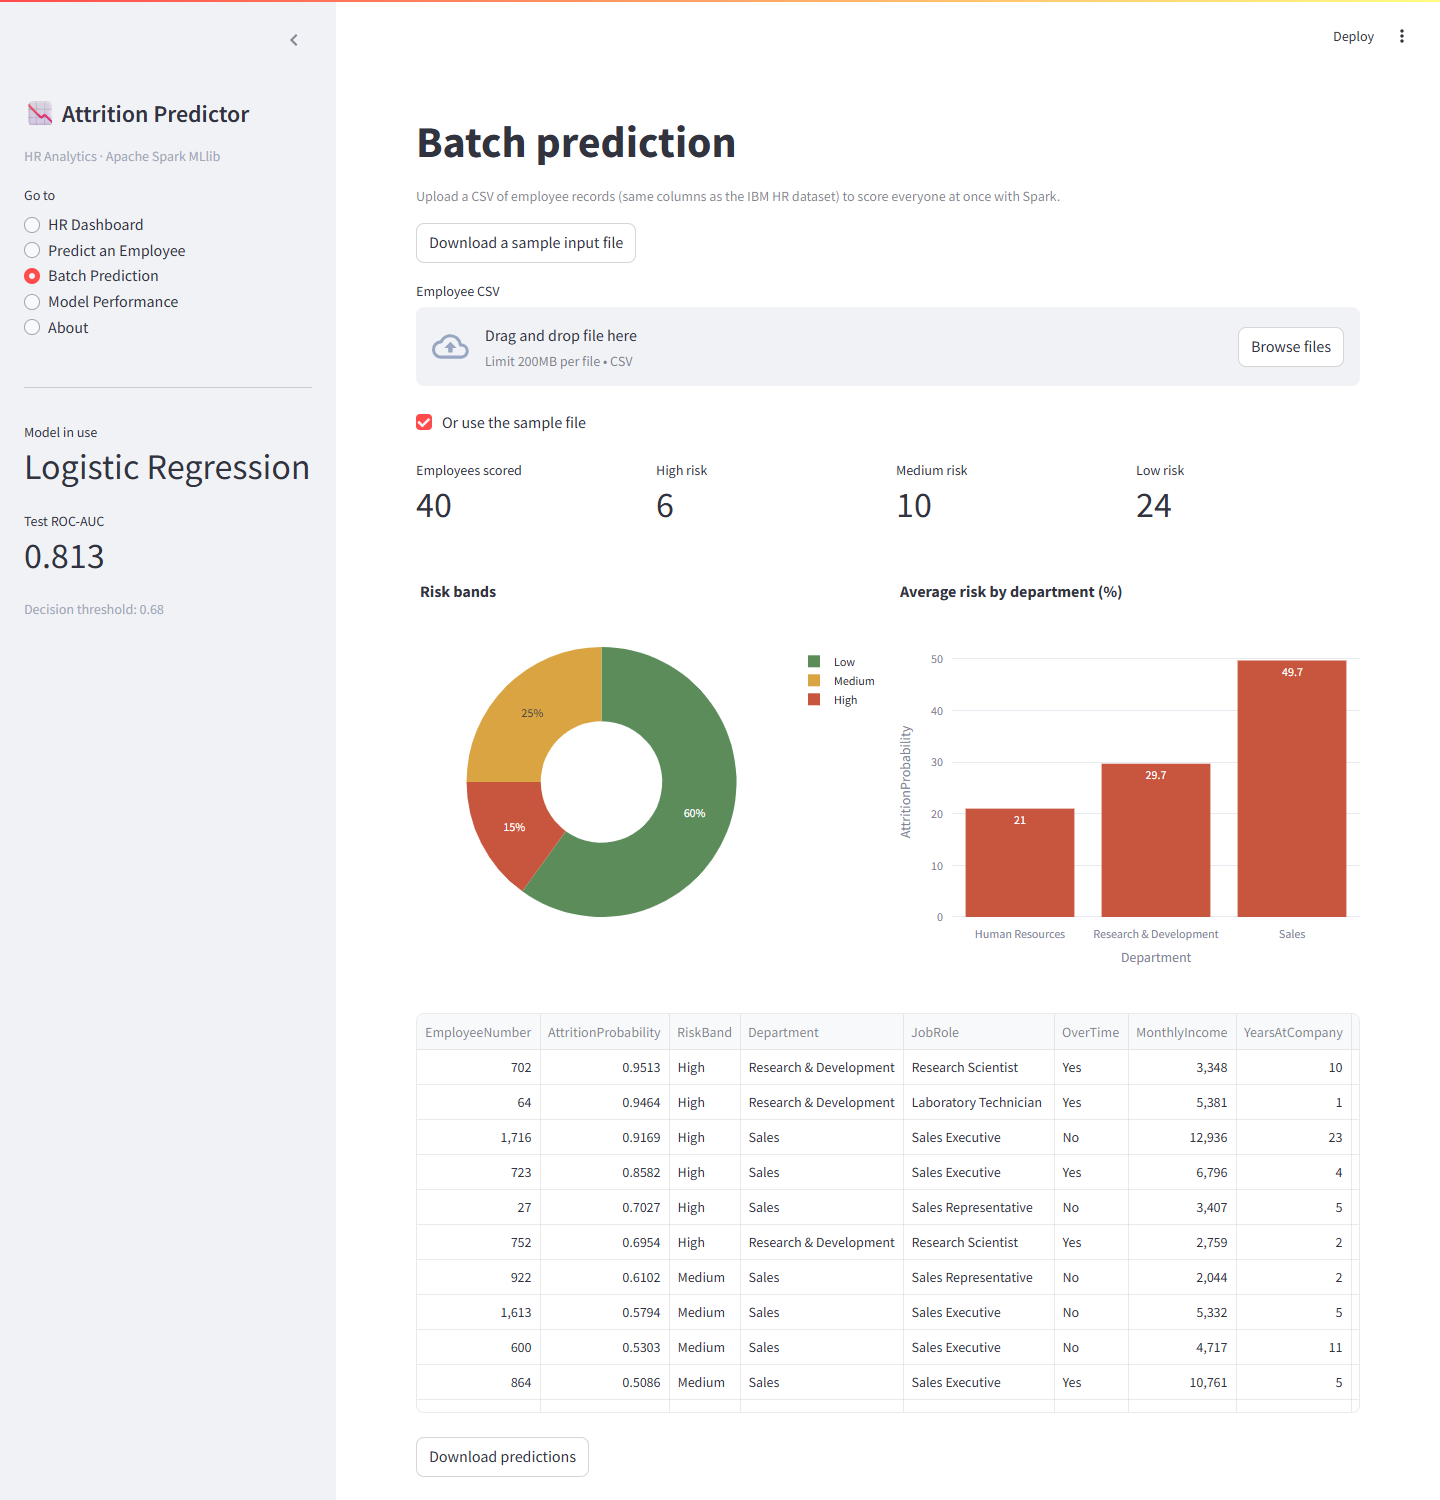
\includegraphics[width=\textwidth,height=0.75\textheight,keepaspectratio]{figures/app_04_batch.png}
\caption{Batch Prediction page}
\end{figure}}{}

\IfFileExists{figures/app_05_performance.png}{%
\begin{figure}[H]
\centering
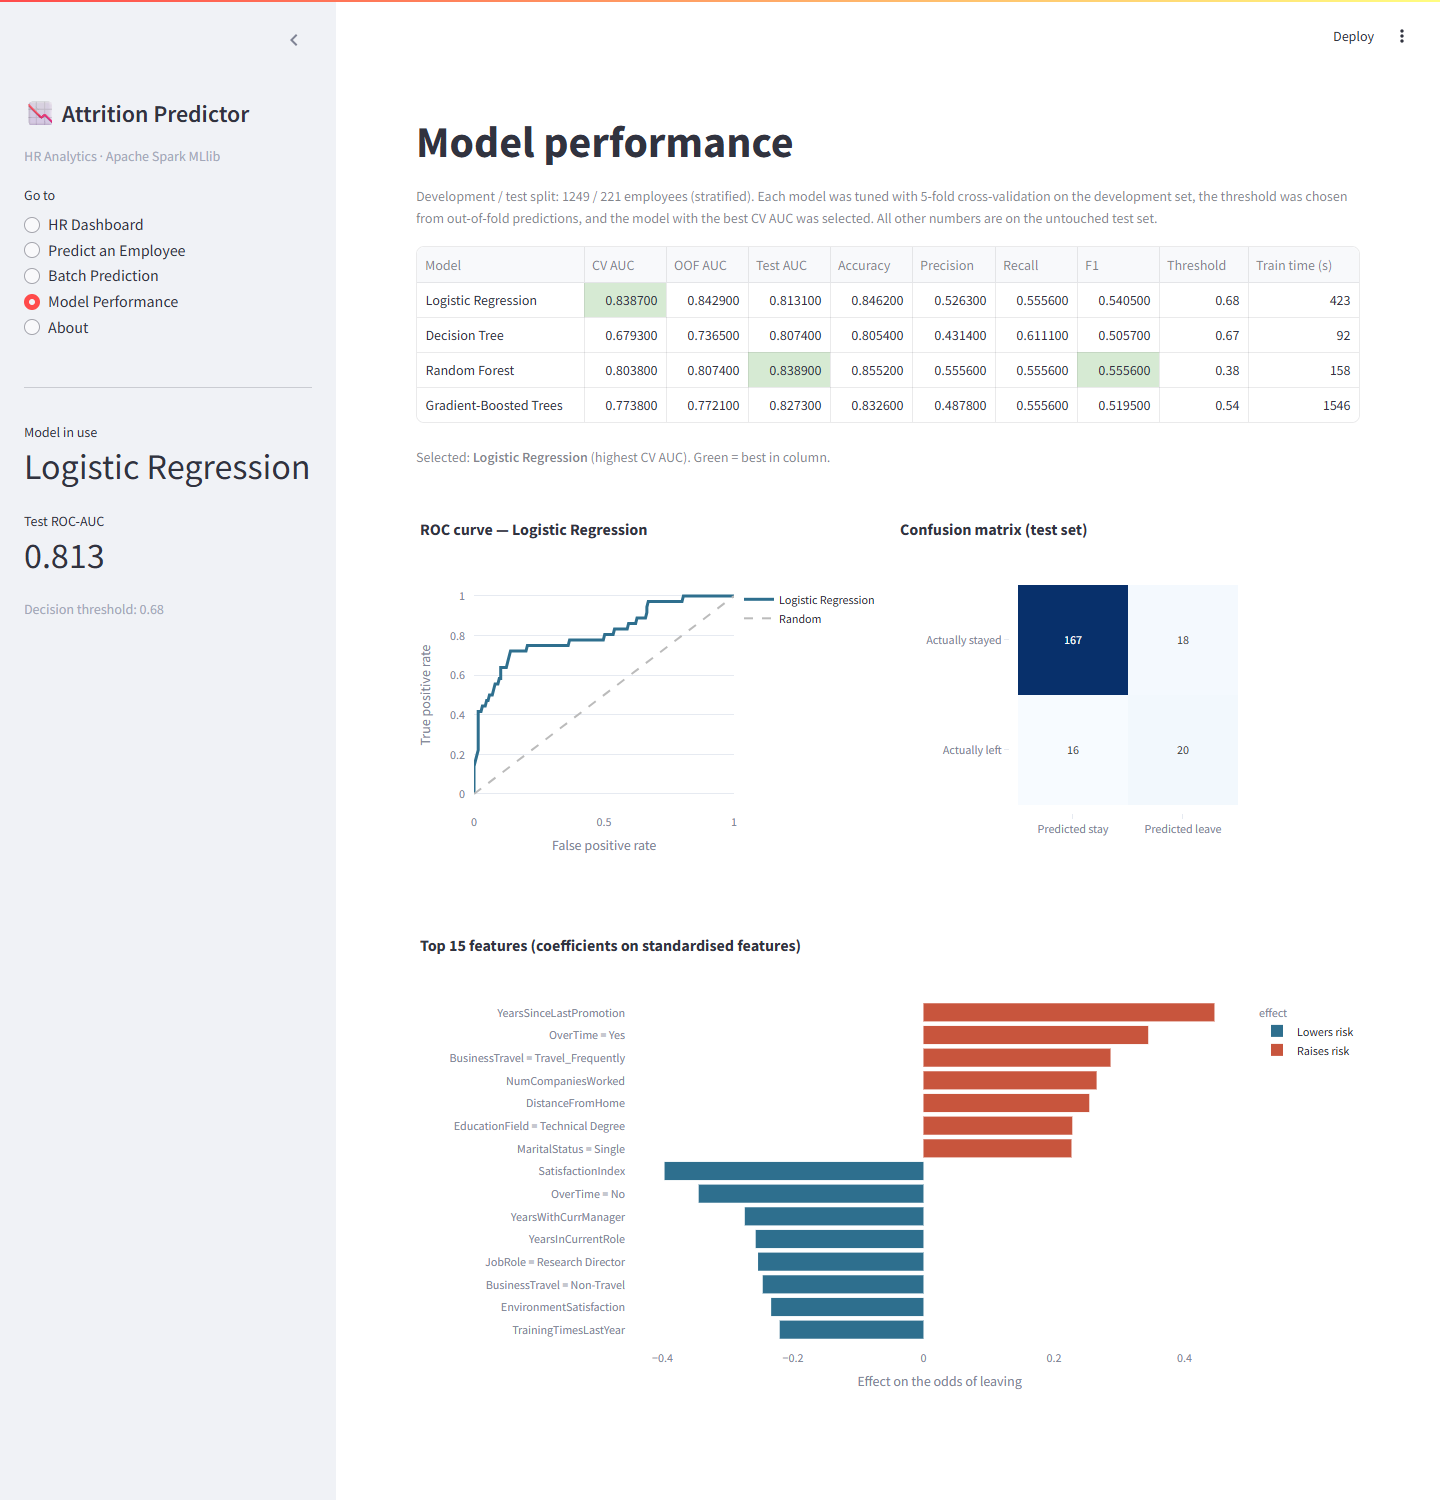
\includegraphics[width=\textwidth,height=0.75\textheight,keepaspectratio]{figures/app_05_performance.png}
\caption{Model Performance page}
\end{figure}}{}

\chapter{How to Run the Project}
\label{app:run}

\textbf{Prerequisites:} Python 3.11, Java 17. On Windows, \texttt{winutils.exe} and \texttt{hadoop.dll} (Hadoop 3.3) in \texttt{\%USERPROFILE\%\textbackslash hadoop\textbackslash bin}, which Spark needs to save models.

\begin{lstlisting}
git clone https://github.com/varunmundhada/employee-attrition-prediction.git
cd employee-attrition-prediction
python -m venv .venv
.venv\Scripts\activate          # Linux / macOS: source .venv/bin/activate
pip install -r requirements.txt

python -m src.eda               # analysis + charts
python -m src.train             # train, compare, save best model
python -m pytest -q             # tests
streamlit run app/streamlit_app.py   # open http://localhost:8501

python -m src.predict data/sample_employees.csv out.csv   # CLI scoring
python -m src.scale_benchmark                            # scalability test
\end{lstlisting}

On Windows the batch files \texttt{setup.bat}, \texttt{run\_pipeline.bat} and \texttt{run\_app.bat} run the same steps.

% Save the Turnitin similarity report as plagiarism_report_final.pdf in this folder.
\IfFileExists{plagiarism_report_final.pdf}{%
\includepdf[
pages=1, scale = 0.7, offset=0 -1cm, pagecommand={\chapter{Plagiarism Report}\thispagestyle{fancy}}
]{plagiarism_report_final.pdf}
\includepdf[
pages=2-, scale=0.7, offset=0 -1cm,pagecommand={\thispagestyle{fancy}}
]{plagiarism_report_final.pdf}}{%
\chapter{Plagiarism Report}
\placeholderpage{Plagiarism Report}{Turnitin similarity report for this document, to be inserted after the final draft is checked.}}

% Save the AI similarity report as ai_report_final.pdf in this folder.
\IfFileExists{ai_report_final.pdf}{%
\includepdf[
pages=1,
scale=0.7, offset=0 -1cm, pagecommand={\chapter{AI Similarity Report}\thispagestyle{fancy}}
]{ai_report_final.pdf}
\includepdf[
pages=2-, scale=0.7, offset=0 -1cm,pagecommand={\thispagestyle{fancy}}
]{ai_report_final.pdf}}{%
\chapter{AI Similarity Report}
\placeholderpage{AI Similarity Report}{AI similarity report for this document, to be inserted after the final draft is checked.}}

\end{document}
